\documentclass[12pt, a4paper]{report}

\usepackage[italian]{babel}

\usepackage[tmargin=3cm,rmargin=1in,lmargin=1in,margin=0.85in,bmargin=3cm]{geometry}
\usepackage{amsmath,amsfonts,amsthm,amssymb,mathtools}
\usepackage{bookmark}
\usepackage{enumitem}
\usepackage{hyperref}
\hypersetup{
	colorlinks=true,
  allcolors=fg,
	bookmarksnumbered=true,
	bookmarksopen=true
}
\usepackage[most,many,breakable]{tcolorbox}
\usepackage{xcolor}
\usepackage{algorithm}
\usepackage{algpseudocode}
\usepackage{caption}
\usepackage{subcaption}
\usepackage{float}
\usepackage{tikz}
\usepackage{tikz-cd}
\usepackage{tikzsymbols}
\usetikzlibrary{patterns, shapes.misc}
\usepackage{xpatch}% to patch \cancel
\usepackage[bottom]{footmisc}
\usepackage{graphbox}

\algdef{SE}[DOWHILE]{Do}{DoWhile}{\algorithmicdo}[1]{\algorithmicwhile\ #1}%


\definecolor{bg}{HTML}{F2F2F2}
\definecolor{fg}{HTML}{282828}

\setlength{\parindent}{0pt}

% change default chapter distance
\makeatletter
% --- Patch \chapter
\patchcmd{\@makechapterhead}{50\p@}{\chapheadtopskip}{}{}% Space from top of page to CHAPTER X
\patchcmd{\@makechapterhead}{20\p@}{\chapheadsep}{}{}% Space between CHAPTER X and CHAPTER TITLE
\patchcmd{\@makechapterhead}{40\p@}{\chapheadbelowskip}{}{}% Space between CHAPTER TITLE and text
% --- Patch \chapter*
\patchcmd{\@makeschapterhead}{50\p@}{\chapheadtopskip}{}{}% Space from top of page to CHAPTER TITLE
\patchcmd{\@makeschapterhead}{40\p@}{\chapheadbelowskip}{}{}% SPace between CHAPTER TITLE and text
\makeatother
% Set new lengths
\newlength{\chapheadtopskip}\setlength{\chapheadtopskip}{0pt}
\newlength{\chapheadsep}\setlength{\chapheadsep}{15pt}
\newlength{\chapheadbelowskip}\setlength{\chapheadbelowskip}{25pt}

% deliminators
\DeclarePairedDelimiter{\abs}{\lvert}{\rvert}
\DeclarePairedDelimiter{\norm}{\lVert}{\rVert}

\DeclarePairedDelimiter{\ceil}{\lceil}{\rceil}
\DeclarePairedDelimiter{\floor}{\lfloor}{\rfloor}
\DeclarePairedDelimiter{\round}{\lfloor}{\rceil}

\let\oldleq\leq
\let\oldgeq\geq
\renewcommand{\leq}{\leqslant}
\renewcommand{\geq}{\geqslant}

\usepackage{titletoc}
\contentsmargin{0cm}
\titlecontents{part}[-1pc]
{\addvspace{50pt}%
	\begin{tikzpicture}[remember picture, overlay]%
		\draw[fill=fg!85,draw=fg!85] (-4.5,-0.2) rectangle (-0.15,0.55);%
		\pgftext[left,x=-1.6cm,y=0.15cm]{\color{bg}\Large Part}%
	\end{tikzpicture}\color{fg}\large}
{}
{}
{}
\titlecontents{chapter}[5pc]
{\addvspace{30pt}%
	\begin{tikzpicture}[remember picture, overlay]%
		\draw[fill=fg!85,draw=fg!85] (-3.6,-0.2) rectangle (-0.12,0.55);%
		\pgftext[left,x=-3.5cm,y=0.15cm]{\color{bg}\Large Chapter\ \thecontentslabel}%
	\end{tikzpicture}\color{fg}\large}%
{}
{}
{\;\titlerule\;\large Page \thecontentspage
	\begin{tikzpicture}[remember picture, overlay]
		\draw[fill=fg,draw=fg] (4pt,0.2pt) rectangle (4,0.2pt);
	\end{tikzpicture}}%
\titlecontents{section}[5pc]
{\addvspace{2pt}}
{\contentslabel[\thecontentslabel]{2pc}}
{}
{\hfill\small \thecontentspage}
[]
\titlecontents{subsection}[5pc]
{\addvspace{2pt}}
{\scriptsize$\bullet$\quad\small}
{}
{\hfill\small}
[]

\makeatletter
\renewcommand{\tableofcontents}{%
	\chapter*{%
	  \vspace*{-20\p@}%
	  \begin{tikzpicture}[remember picture, overlay]%
		  \pgftext[right,x=16.7cm,y=0.2cm]{\color{fg!85}\Huge \contentsname}%
		  \draw[fill=fg!85,draw=fg!85] (14.6,-0.65) rectangle (20,1);%
		  \clip (14.6,-0.65) rectangle (20,1);
		  \pgftext[right,x=16.7cm,y=0.2cm]{\color{bg}\Huge \contentsname}%
	  \end{tikzpicture}}%
	\@starttoc{toc}}
\makeatother

\usepackage[italian]{babel}

\title{\Huge{Implementazione distribuita dell'algoritmo Flood-Fill}}
\author{\Large{\textit{Tam Gabriele, Merlo Filippo}}}
\date{\today}

\begin{document}

\maketitle

\newpage
\pdfbookmark[section]{\contentsname}{toc}
\tableofcontents
\pagebreak

\begin{abstract} L'algoritmo Flood-Fill \`e una tecnica utilizzata per ricolorare aree connesse in strutture bidimensionali, comunemente applicato in grafica computerizzata. L'obiettivo di questo progetto \`e l'implementazione distribuita dell'algoritmo, con una rappresentazione dove ogni pixel di un'immagine \`e trattato come un nodo di una rete distribuita. In questo contesto, emergono sfide legate alla comunicazione tra nodi, alla consistenza dello stato, alla gestione delle richieste concorrenti e alla tolleranza ai guasti.

Nel documento viene proposto un approccio basato su una partizione dei nodi in cluster, gestiti da nodi leader, e su una rete overlay tra leader per facilitare operazioni di merge e coordinamento. Viene implementato un sistema che garantisce scalabilit\`a, robustezza e consistenza utilizzando un time-server che gestisce i timestamp per l'ordinamento degli eventi e un database condiviso per la sincronizzazione globale. Inoltre, il sistema \`e progettato per essere resiliente ai guasti, con meccanismi di elezione di nuovi leader e recupero dei nodi. I risultati mostrano che la soluzione proposta \`e efficiente e adatta a reti di grandi dimensioni. \end{abstract}

\chapter{Introduzione}

In questo capitolo viene descritto il problema principale affrontato dal progetto, insieme a una panoramica della soluzione proposta. L'obiettivo \`e sviluppare una versione distribuita dell'algoritmo \emph{Flood-Fill}, che permette di ricolorare aree connesse in una struttura bidimensionale, come un'immagine digitale, dove ogni pixel \`e rappresentato da un nodo della rete distribuita. Questo scenario introduce sfide legate alla comunicazione tra nodi, alla gestione delle operazioni concorrenti e alla tolleranza ai guasti, tutti aspetti che devono essere gestiti in modo efficiente.

\section{Descrizione del problema}

Il problema consiste nel ricolorare un'area connessa di una matrice bidimensionale $img[N][M]$, dove ogni elemento $img[i][j]$\footnote{con $0 \le i < N$ e $0 \le j < M$} rappresenta il colore di un pixel in posizione $(i,j)$. Dato un pixel iniziale in posizione \texttt{(x, y)} e un nuovo colore \texttt{newColor}, l'obiettivo \`e rimpiazzare il colore del pixel selezionato e di tutti i pixel adiacenti che condividono lo stesso colore iniziale con \texttt{newColor} (vedi Fig.~\ref{fig:esempio_nodi}). Questa ricolorazione deve propagarsi attraverso nodi adiacenti, in tutte le direzioni (orizzontale, verticale, diagonale).

\begin{figure}[H]
    \captionsetup{justification=centering, margin=2cm}
    \centering
    \begin{subfigure}{0.48\textwidth}
        \captionsetup{justification=centering, margin=1cm}
        \centering
        \begin{tikzpicture}
    \fill[black!30] (1, 5) rectangle ++(1,1);
    \fill[black!30] (3, 5) rectangle ++(1,1);
    \fill[black!30] (2, 4) rectangle ++(1,1);
    \fill[black!30] (2, 6) rectangle ++(1,1);
    \fill[black!30] (3, 6) rectangle ++(1,1);
    \fill[black!30] (3, 4) rectangle ++(1,1);
    \fill[black!30] (1, 6) rectangle ++(1,1);
    \fill[black!30] (1, 4) rectangle ++(1,1);

    \fill[red!30] (2, 5) rectangle ++(1,1);

    \draw[thick, black] (1, 5) rectangle ++(1,1);
    \draw[thick, black] (3, 5) rectangle ++(1,1);
    \draw[thick, black] (2, 4) rectangle ++(1,1);
    \draw[thick, black] (2, 6) rectangle ++(1,1);
    \draw[thick, black] (3, 6) rectangle ++(1,1);
    \draw[thick, black] (3, 4) rectangle ++(1,1);
    \draw[thick, black] (1, 6) rectangle ++(1,1);
    \draw[thick, black] (1, 4) rectangle ++(1,1);

    \draw[thick, red] (2, 5) rectangle ++(1,1);
    
    % Draw the grid and add colored letters
    \node[fill=red!60, text=white, font=\bfseries] at (0.5, 6.5) {R}; 
    \node[fill=red!60, text=white, font=\bfseries] at (1.5, 6.5) {R}; 
    \node[fill=blue!60, text=white, font=\bfseries] at (2.5, 6.5) {B}; 
    \node[fill=cyan!60, text=white, font=\bfseries] at (3.5, 6.5) {C}; 
    \node[fill=cyan!60, text=white, font=\bfseries] at (4.5, 6.5) {C};
    
    \node[fill=red!60, text=white, font=\bfseries] at (0.5, 5.5) {R}; 
    \node[fill=red!60, text=white, font=\bfseries] at (1.5, 5.5) {R}; 
    \node[fill=blue!60, text=white, font=\bfseries] at (2.5, 5.5) {B}; 
    \node[fill=cyan!60, text=white, font=\bfseries] at (3.5, 5.5) {C}; 
    \node[fill=cyan!60, text=white, font=\bfseries] at (4.5, 5.5) {C};
    
    \node[fill=red!60, text=white, font=\bfseries] at (0.5, 4.5) {R}; 
    \node[fill=red!60, text=white, font=\bfseries] at (1.5, 4.5) {R}; 
    \node[fill=blue!60, text=white, font=\bfseries] at (2.5, 4.5) {B};  % Nodo centrale
    \node[fill=green!60, text=white, font=\bfseries] at (3.5, 4.5) {G}; 
    \node[fill=green!60, text=white, font=\bfseries] at (4.5, 4.5) {G};
    
    \node[fill=red!60, text=white, font=\bfseries] at (0.5, 3.5) {R}; 
    \node[fill=red!60, text=white, font=\bfseries] at (1.5, 3.5) {R}; 
    \node[fill=blue!60, text=white, font=\bfseries] at (2.5, 3.5) {B}; % Vicino dello stesso colore
    \node[fill=green!60, text=white, font=\bfseries] at (3.5, 3.5) {G}; 
    \node[fill=green!60, text=white, font=\bfseries] at (4.5, 3.5) {G};
    
    \node[fill=blue!60, text=white, font=\bfseries] at (0.5, 2.5) {B}; 
    \node[fill=blue!60, text=white, font=\bfseries] at (1.5, 2.5) {B}; % Vicino dello stesso colore
    \node[fill=blue!60, text=white, font=\bfseries] at (2.5, 2.5) {B}; % Vicino dello stesso colore
    \node[fill=green!60, text=white, font=\bfseries] at (3.5, 2.5) {G}; 
    \node[fill=green!60, text=white, font=\bfseries] at (4.5, 2.5) {G};
\end{tikzpicture}
        \caption{L'area evidenziata in grigio sono i nodi adiancenti.}
        \label{fig:nodi_adiacenti}
    \end{subfigure}
    \hfill
    \begin{subfigure}{0.48\textwidth}
        \captionsetup{justification=centering, margin=1cm}
        \centering
        \begin{tikzpicture}
    \fill[orange!30] (2, 6) rectangle ++(1,1);
    \fill[red!30] (2, 5) rectangle ++(1,1);
    \fill[orange!30] (2, 4) rectangle ++(1,1);
    \fill[orange!30] (2, 3) rectangle ++(1,1);
    \fill[orange!30] (2, 2) rectangle ++(1,1);
    \fill[orange!30] (1, 2) rectangle ++(1,1);
    \fill[orange!30] (0, 2) rectangle ++(1,1);

    \draw[thick, black] (2, 6) rectangle ++(1,1);
    \draw[thick, black] (2, 4) rectangle ++(1,1);
    \draw[thick, black] (2, 3) rectangle ++(1,1);
    \draw[thick, black] (2, 2) rectangle ++(1,1);
    \draw[thick, black] (1, 2) rectangle ++(1,1);
    \draw[thick, black] (0, 2) rectangle ++(1,1);
    
    \draw[thick, red] (2, 5) rectangle ++(1,1);

    
    % Draw the grid and add colored letters
    \node[fill=red!60, text=white, font=\bfseries] at (0.5, 6.5) {R}; 
    \node[fill=red!60, text=white, font=\bfseries] at (1.5, 6.5) {R}; 
    \node[fill=blue!60, text=white, font=\bfseries] at (2.5, 6.5) {B}; 
    \node[fill=cyan!60, text=white, font=\bfseries] at (3.5, 6.5) {C}; 
    \node[fill=cyan!60, text=white, font=\bfseries] at (4.5, 6.5) {C};
    
    \node[fill=red!60, text=white, font=\bfseries] at (0.5, 5.5) {R}; 
    \node[fill=red!60, text=white, font=\bfseries] at (1.5, 5.5) {R}; 
    \node[fill=blue!60, text=white, font=\bfseries] at (2.5, 5.5) {B}; 
    \node[fill=cyan!60, text=white, font=\bfseries] at (3.5, 5.5) {C}; 
    \node[fill=cyan!60, text=white, font=\bfseries] at (4.5, 5.5) {C};
    
    \node[fill=red!60, text=white, font=\bfseries] at (0.5, 4.5) {R}; 
    \node[fill=red!60, text=white, font=\bfseries] at (1.5, 4.5) {R}; 
    \node[fill=blue!60, text=white, font=\bfseries] at (2.5, 4.5) {B};  % Nodo centrale
    \node[fill=green!60, text=white, font=\bfseries] at (3.5, 4.5) {G}; 
    \node[fill=green!60, text=white, font=\bfseries] at (4.5, 4.5) {G};
    
    \node[fill=red!60, text=white, font=\bfseries] at (0.5, 3.5) {R}; 
    \node[fill=red!60, text=white, font=\bfseries] at (1.5, 3.5) {R}; 
    \node[fill=blue!60, text=white, font=\bfseries] at (2.5, 3.5) {B}; % Vicino dello stesso colore
    \node[fill=green!60, text=white, font=\bfseries] at (3.5, 3.5) {G}; 
    \node[fill=green!60, text=white, font=\bfseries] at (4.5, 3.5) {G};
    
    \node[fill=blue!60, text=white, font=\bfseries] at (0.5, 2.5) {B}; 
    \node[fill=blue!60, text=white, font=\bfseries] at (1.5, 2.5) {B}; % Vicino dello stesso colore
    \node[fill=blue!60, text=white, font=\bfseries] at (2.5, 2.5) {B}; % Vicino dello stesso colore
    \node[fill=green!60, text=white, font=\bfseries] at (3.5, 2.5) {G}; 
    \node[fill=green!60, text=white, font=\bfseries] at (4.5, 2.5) {G};
\end{tikzpicture}
        \caption{L'area evidenziata in giallo sono i nodi del cluster.}
        \label{fig:nodi_cluster}
    \end{subfigure}
    \caption{A partire dal nodo scelto (evidenziato di rosso), si mostrano i suoi nodi adiacenti (\ref{fig:nodi_adiacenti}) e quelli del cluster (\ref{fig:nodi_cluster}).}
    \label{fig:esempio_nodi}
\end{figure}


Ogni nodo della rete \`e responsabile di un pixel e collabora con i nodi adiacenti per completare l'operazione di ricolorazione.

\section{Terminologia}

Per una migliore comprensione e per evitare ambiguit\`a, vengono definiti alcuni termini chiave:

\begin{itemize}[label=]
    \item \textbf{Nodo}: un processo autonomo nella rete, responsabile di un singolo pixel dell'immagine.
    \item \textbf{Colore}: la propriet\`a associata a ciascun nodo, che rappresenta lo stato corrente (colore) del pixel.
    \item \textbf{Nodi adiacenti}: i nodi che si trovano in posizioni adiacenti nella matrice, ovvero collegati orizzontalmente, verticalmente o diagonalmente.
    \item \textbf{Cluster}: un gruppo di nodi, i quali condividono lo stesso colore e sono connessi tra loro. Nel nostro approccio di soluzione, i cluster vengono gestiti a livello locale per ottimizzare le operazioni di ricolorazione.
    \item \textbf{Nodo Leader}: il nodo designato all'interno di un cluster per coordinare le operazioni globali, come l'avvio delle ricolorazioni e la fusione con altri cluster.
    \item \textbf{Ricolorazione/Cambio di colore}: l'operazione di aggiornamento del colore di un cluster innescata dalla scelta di un nodo iniziale.
    \item \textbf{Fusione/Unione/Merge di cluster}: l'unione di due o pi\`u cluster adiacenti quando questi condividono lo stesso colore a seguito di operazioni di ricolorazione, gestita dai rispettivi nodi leader.
\end{itemize}

\section{Struttura complessiva dell'implementazione}

Il sistema \`e strutturato come una rete di nodi, i quali sono organizzati in cluster basati sul colore condiviso. Ogni cluster \`e gestito da un \emph{nodo leader}, il quale si occupa di coordinare le operazioni sia interne che esterne al cluster: la gestione delle operazioni distribuite richiede una comunicazione efficiente, che \`e garantita tramite una rete overlay tra i leader dei cluster e l'uso di un server centrale per mantenere lo stato globale del sistema.

\section{Caratteristiche del sistema distribuito}

Il sistema implementa diverse funzionalit\`a proprie dei sistemi distribuiti:
\begin{itemize}
    \item \textbf{Trasparenza nella comunicazione}: ogni nodo comunica direttamente con i nodi adiacenti, o con il leader del cluster, senza necessit\`a di conoscere la topologia completa.
    \item \textbf{Consistenza}: la consistenza globale del sistema \`e garantita tramite l'associazione delle operazioni a \textbf{timestamps}, grazie ai quali risulta possibile ordinarle correttamente, evitando possibili conflitti dovuti alla concorrenza.
    \item \textbf{Tolleranza ai guasti}: meccanismi di failover assicurano che il sistema possa continuare a funzionare anche in caso di guasti di singoli nodi (sia normali che leader).
\end{itemize}

\section{Algoritmi implementati}

Il sistema utilizza vari algoritmi per garantire la corretta esecuzione dell'algoritmo distribuito di Flood-Fill:
\begin{itemize}
    \item \textbf{Algoritmo di cambio colore}: i nodi comunicano col leader per avviare la propagazione della ricolorazione. Il leader coordina l'operazione per evitare conflitti tra pi\`u richieste.
    \item \textbf{Algoritmo di merge dei cluster}: quando due cluster adiacenti vengono ricolorati con lo stesso colore, i leader coordinano l'unione dei cluster e la gestione dei loro confini.
    \item \textbf{Algoritmo di gestione dei fallimenti}: include procedure per la rielezione dei leader e la gestione dei nodi disconnessi o falliti.
\end{itemize}

\section{Piano di test}

Il sistema sar\`a testato simulando scenari di ricolorazione su immagini di grandi dimensioni: i test valuteranno la robustezza del sistema in situazioni di concorrenza (pi\`u richieste simultanee di cambio colore) e in presenza di guasti di nodi leader o normali. L'attenzione sar\`a posta sulla consistenza delle operazioni distribuite.

\section{Programma di sviluppo}

Il progetto si articola in diverse fasi:
\begin{enumerate}
    \item \textbf{Fase di progettazione}: definizione dell'architettura del sistema e degli algoritmi distribuiti.
    \item \textbf{Fase di implementazione}: sviluppo dei componenti principali, tra cui i nodi normali, i nodi leader e il server centrale, con particolare attenzione alla gestione della consistenza e dei guasti.
    \item \textbf{Fase di testing}: esecuzione di test per verificare il corretto funzionamento del sistema.
\end{enumerate}

\chapter{Analisi}\label{chapter:analisi}

In questo capitolo vengono descritti nel dettaglio i requisiti funzionali e non funzionali di una soluzione per l'implementazione distribuita dell'algoritmo \emph{Flood-Fill}. Questi requisiti guidano lo sviluppo del sistema, specificando le funzionalit\`a richieste e le qualit\`a desiderabili, insieme alle assunzioni e ai vincoli considerati durante l'implementazione.

\section{Requisiti Funzionali}

I requisiti funzionali definiscono le operazioni principali che il sistema deve offrire, specificando come devono essere gestiti input e output, e l'effetto atteso per ogni funzione.

\begin{enumerate}
    \item \textbf{Operazione di colorazione distribuita}: il sistema deve permettere a un nodo di iniziare un'operazione di ricolorazione, propagando il nuovo colore a tutti i nodi adiacenti che condividono lo stesso colore iniziale.

    \item \textbf{Gestione di richieste concorrenti}: il sistema deve essere in grado di gestire pi\`u richieste di ricolorazione simultanee provenienti da nodi diversi, garantendo un comportamento deterministico e la corretta risoluzione dei conflitti.

    \item \textbf{Comunicazione tra nodi}: i nodi devono essere in grado di scambiarsi messaggi con i loro vicini adiacenti per sincronizzare lo stato e coordinare le operazioni di colorazione. Ogni nodo deve mantenere aggiornate le informazioni relative ai vicini e al leader del proprio cluster.

    \item \textbf{Fusione dei cluster}: quando due cluster adiacenti diventano dello stesso colore a seguito di una ricolorazione, il sistema deve unificarli in uno solo. Il nodo leader del cluster risultante deve gestire le future operazioni di ricolorazione e fusione.

    \item \textbf{Tolleranza ai guasti}: il sistema deve essere in grado di gestire il fallimento di singoli nodi, sia leader che normali, garantendo che il resto del cluster continui a operare correttamente. Devono essere previsti meccanismi di failover per la rielezione dei leader.

    \item \textbf{Consistenza globale}: il sistema deve mantenere una consistenza globale dello stato, garantendo che tutti i nodi di un cluster condividano lo stesso colore dopo ogni operazione di ricolorazione o fusione.
\end{enumerate}

\newpage
\section{Requisiti Non Funzionali}

I requisiti non funzionali riguardano le qualit\`a desiderabili del sistema, tra cui prestazioni, sicurezza e tolleranza ai guasti. Essi descrivono le caratteristiche che devono essere garantite durante l'implementazione.

\begin{enumerate}
    \item \textbf{Scalabilit\`a}: il sistema deve essere in grado di supportare un elevato numero di nodi, mantenendo buone prestazioni anche con una rete distribuita estesa.

    \item \textbf{Efficienza delle comunicazioni}: il numero di messaggi scambiati tra i nodi deve essere minimizzato per evitare sovraccarichi di rete. L'algoritmo di ricolorazione e fusione deve utilizzare una comunicazione locale, limitata ai vicini diretti, salvo necessit\`a di sincronizzazione globale.

    \item \textbf{Robustezza e affidabilit\`a}: il sistema deve essere resiliente ai guasti e garantire il recupero rapido dopo il fallimento di uno o pi\`u nodi, inclusi i nodi leader. Deve essere possibile continuare le operazioni anche in caso di guasti isolati.

    \item \textbf{Consistenza}: il sistema deve garantire la consistenza dello stato anche in presenza di richieste concorrenti o di fallimenti.

\end{enumerate}

\section{Assunzioni e Vincoli}

Le seguenti assunzioni e vincoli sono stati considerati per l'implementazione del sistema distribuito:

\begin{itemize}
    \item \textbf{Topologia della rete}: si assume che la rete sottostante sia affidabile, ossia che i messaggi inviati tra nodi adiacenti vengano consegnati correttamente entro un tempo limite ragionevole.

    % \item \textbf{Modalit\`a asincrona}: si assume che i nodi operino in maniera asincrona, senza un clock globale sincronizzato. Le operazioni locali e la comunicazione tra nodi devono avvenire in maniera indipendente.

    \item \textbf{Fallimenti dei nodi}: si assume che i nodi possano fallire in modalit\`a \emph{crash}, ossia che possano smettere di funzionare senza comportamento bizantino (comportamenti non affidabili o malevoli).

    \item \textbf{Conoscenza locale}: ogni nodo ha una conoscenza locale limitata dei propri vicini e del leader del proprio cluster. Nessun nodo ha una visione globale dell'intera rete o di tutti i cluster.

    \item \textbf{Inizializzazione dei nodi}: al momento dell'avvio, ogni nodo conosce solo le proprie coordinate all'interno della matrice dell'immagine e il colore iniziale del pixel che rappresenta. La formazione dei cluster e la gestione della rete overlay avvengono durante la fase di esecuzione.

\end{itemize}

\chapter{Progettazione del sistema}

In questo capitolo viene presentata la progettazione del sistema: verranno analizzate le possibili soluzioni, spiegando i vantaggi e gli svantaggi di ciascuna e successivamente verr\`a presentata la soluzione scelta, descrivendone architettura, componenti ed algoritmi utilizzati.

\section{Analisi delle possibili soluzioni}

Sono stati considerati due principali approcci:

\begin{enumerate}
    \item \textbf{Comunicazione diretta tra nodi}: ogni nodo comunica unicamente coi propri nodi adiacenti per propagare il cambiamento di colore.
    \item \textbf{Partizionamento del grafo e elezione di nodi leader}: il grafo viene suddiviso in cluster, ciascuno gestito dal proprio nodo leader che ne coordina operazioni (e.g. ricolorazione) ed organizzazione (e.g. fallimento di nodi, merge, $\ldots$).
\end{enumerate}

\subsubsection{1. Comunicazione diretta tra nodi}

\paragraph{Descrizione generale}
\begin{flushleft}
In questo approccio, ogni nodo mantiene informazioni locali e comunica direttamente con i nodi adiacenti. Quando un nodo cambia colore, l'operazione di ricolorazione viene unicamente propagata ai nodi adiacenti che condividono lo stesso colore, creando una diffusione a cascata.
\end{flushleft}

\paragraph{Vantaggi}

\begin{itemize}
    \item \textbf{Semplicit\`a}: l'implementazione \`e relativamente semplice poich\'e ogni nodo gestisce solo informazioni locali.
    \item \textbf{Assenza di punti singoli di fallimento}: non esistono nodi centrali il cui fallimento compromette l'intero sistema.
\end{itemize}

\paragraph{Svantaggi}

\begin{itemize}
    \item \textbf{Scalabilit\`a limitata}: l'elevato numero di messaggi scambiati pu\`o diventare insostenibile in reti di grandi dimensioni.
    \item \textbf{Concorrenza non deterministica}: difficolt\`a nel gestire richieste concorrenti in modo deterministico.
    \item \textbf{Gestione dei fallimenti complessa}: la mancanza di una visione globale rende difficile il recupero da guasti.
\end{itemize}

\subsubsection{2. Partizionamento del grafo e nodi leader}

\paragraph{Descrizione generale}
\begin{flushleft}
In questo approccio, il grafo \`e partizionato in cluster, ognuno dei quali \`e gestito dal proprio \textbf{nodo leader} responsabile della gestione dello stato e delle decisioni per il cluster. I nodi normali delegano le decisioni al leader, riducendo la complessit\`a locale.
\end{flushleft}
\paragraph{Vantaggi}

\begin{itemize}
    \item \textbf{Consistenza migliorata}: la centralizzazione delle decisioni nel leader migliora la consistenza del sistema.
    \item \textbf{Gestione efficiente della concorrenza}: il leader gestisce richieste concorrenti in modo ordinato.
    \item \textbf{Scalabilit\`a}: partizionando il grafo si riduce la complessit\`a in cluster pi\`u piccoli.
\end{itemize}

\paragraph{Svantaggi}

\begin{itemize}
    \item \textbf{Punti singoli di fallimento}: il fallimento del leader pu\`o compromettere il funzionamento del cluster.
    \item \textbf{Complessit\`a aggiuntiva}: l'implementazione di leader, algoritmi di elezione e meccanismi di consenso aggiungono complessit\`a.
    \item \textbf{Possibili colli di bottiglia}: il leader pu\`o diventare un collo di bottiglia in cluster molto attivi.
\end{itemize}

\section{Soluzione proposta}

In questo progetto \`e stato usato come base il secondo approccio appena presentato, il quale \`e stato arricchito di varie scelte implementative atte a limitare al minimo gli svantaggi della soluzione, senza intaccare i vantaggi di essa. L'idea della soluzione qui presentata \`e di trattare ogni cluster come un nodo in un grafo \emph{overlay}: ci\`o permette una gestione efficiente delle comunicazioni tra cluster, semplifica le operazioni di merge e cambio colore, e facilita la consistenza globale del sistema.

\subsection{Idea principale}

L'idea centrale della soluzione \`e la seguente:

\begin{itemize}
    \item \textbf{Trattamento dei cluster come nodi in un grafo overlay}: ogni cluster viene considerato come un singolo nodo in un grafo overlay, dove i nodi rappresentano i leader dei cluster e gli archi rappresentano le adiacenze tra cluster.
    \item \textbf{Comunicazione tra leader}: i nodi leader mantengono una lista dei leader adiacenti nel grafo overlay, permettendo comunicazioni dirette per le operazioni di merge e coordinamento.
    \item \textbf{Utilizzo di un server centrale per la sincronizzazione}: implementazione di un server condiviso per gestione, ordinamento e memorizzazione delle operazioni eseguite. Facilita la consistenza e la gestione delle operazioni concorrenti, fornendo al tempo stesso ridondanza sia delle operazioni eseguite (attraverso un file di log) sia dello stato globale della rete.
    \item \textbf{Rappresentazione dei cluster tramite sotto-grafi}: la visione a grafo della rete permette una creazione e gestione facilitata di sotto-grafi, i quali risultano la struttura ideale per la rappresentazione dei cluster, in quanto condividono le stesse propriet\`a connettive e si adattano alle loro strutture amorfe.
\end{itemize}

\subsection{Setup iniziale}

La fase di setup \`e fondamentale per l'inizializzazione dei parametri dei nodi e la costruzione dei cluster, i quali costituiranno il sistema distribuito. Poiché i nodi inizialmente conoscono solo informazioni su loro stessi, il processo di formazione dei cluster e la scoperta delle connessioni tra di essi viene suddiviso in due fasi, ciascuna con uno scopo specifico:

\begin{itemize}
    \item \textbf{Fase 1: Formazione dei cluster e costruzione del grafo $G$}
    \item \textbf{Fase 2: Scoperta dei cluster adiacenti, costruzione della rete overlay e impostazione dei timestamp}
\end{itemize}

\paragraph{Fase 1: Formazione dei cluster e costruzione del grafo}
Questa fase ha come obiettivo la scoperta dei cluster iniziali e la costruzione del grafo $G$, che rappresenter\`a la rete di comunicazione tra il server e i vari cluster.

\begin{enumerate}
    \item \textbf{Assegnazione dei colori ai nodi:}

    Ogni nodo riceve un colore iniziale scelto casualmente da una palette predefinita. Ogni pixel dell'immagine, di dimensioni $N \times M$, condivider\`a il colore del nodo corrispondente. Questa informazione viene memorizzata localmente da ciascun nodo.

    \item \textbf{Conoscenze iniziali di ciascun nodo:}

    All'inizio di questa fase, ogni nodo conosce solo:
    \begin{itemize}
        \item Le proprie coordinate \texttt{(x, y)} nell'immagine.
        \item Il proprio colore \texttt{color}.
        \item I nodi vicini (\texttt{neighbors}), calcolati in base alle coordinate.
        \item Un identificatore temporaneo \texttt{leaderID}, inizialmente impostato a \texttt{null}.
        \item Una variabile \texttt{visited}, inizialmente impostata a \texttt{False}, che indica se il nodo \`e stato visitato.
    \end{itemize}

    \item \textbf{Avvio della BFS\footnote{Breadth-First Search} da parte del server:}

    Poiché i nodi non possono autonomamente iniziare la BFS, sar\`a il server a gestire questa fase. Il server scorre l'immagine in modo ordinato (da sinistra a destra e dall'alto in basso) e invia un messaggio di avvio al primo nodo non ancora visitato, partendo da $(0, 0)$.

    \begin{itemize}
        \item Il nodo $(0, 0)$ avvia una BFS, visitando tutti i nodi adiacenti con lo stesso colore e aggiornando il proprio \texttt{leaderID}, che diventer\`a lo stesso per tutti i nodi del cluster.
        \item Ogni nodo visitato durante la BFS aggiorna la sua variabile \texttt{visited} a \texttt{True} e propaga il \texttt{leaderID} ai suoi vicini dello stesso cluster.
    \end{itemize}

    \item \textbf{Comunicazione con il server e costruzione del grafo $G$:}

    Alla fine di ogni BFS, il nodo leader del cluster invia un messaggio al server con le seguenti informazioni:
    \begin{itemize}
        \item \texttt{leaderID}: l'identificatore del leader del cluster.
        \item \texttt{color}: il colore del cluster.
    \end{itemize}

    Il server registra queste informazioni e costruisce progressivamente il grafo $G$, che ha come nodo radice il server stesso e come sottografi i cluster rappresentati dai rispettivi leader. Ogni cluster \`e dunque un sottografo di $G$ con il leader come nodo radice del sottografo.

    \item \textbf{Avvio della BFS per gli altri nodi:}

    Il server continua a scorrere l'immagine. Se un nodo \`e gi\`a stato visitato (fa gi\`a parte di un cluster), il server lo ignora e passa al successivo. Se un nodo non \`e stato visitato, avvia una nuova BFS per creare un nuovo cluster. Questo processo continua fino a quando tutti i nodi dell'immagine non sono stati visitati e assegnati a un cluster.

    \item \textbf{Conclusione della fase 1:}

    Al termine della Fase 1, il server ha creato un grafo $G$ completo, con tanti sottografi quante sono le componenti connesse dell'immagine (i cluster), ognuna con un leader identificato.
    
\end{enumerate}

\paragraph{Fase 2: Scoperta dei cluster adiacenti e creazione della rete overlay}

In questa fase, i cluster scoprono i loro vicini e viene costruita una rete overlay tra i leader, con il server che gestisce la sincronizzazione e la comunicazione tra di essi.

\begin{enumerate}
    \item \textbf{Scoperta dei cluster adiacenti:}

    Il server invia un messaggio a ciascun leader per iniziare la scoperta dei cluster adiacenti. Ogni leader invia una richiesta a tutti i nodi del proprio cluster per verificare se i vicini appartengono a un altro cluster, raccogliendo anche gli ID dei nodi.

    \begin{itemize} 
        \item Ogni nodo invia una richiesta ai suoi vicini per ottenere il loro \texttt{leaderID}.
        \item Se un vicino appartiene a un altro cluster (cio\`e, ha un \texttt{leaderID} diverso), il nodo riceve in risposta il \texttt{leaderID} e il colore del vicino. 
        \item Il nodo aggrega queste informazioni (\texttt{leaderID} e colore dei vicini) e le inoltra al leader. 
        \item Il leader riceve così le informazioni complete sui cluster adiacenti (compresi i \texttt{leaderID} e i colori). 
        \item Infine, il leader invia al server una lista completa che include: 
        \begin{itemize} 
            \item Gli ID di tutti i nodi del proprio cluster. 
            \item Una lista dei \texttt{leaderID} dei cluster adiacenti. 
            \item Il colore dei cluster adiacenti. 
        \end{itemize} 
    \end{itemize}

    \item \textbf{Creazione della rete overlay tra i leader:}

    Una volta che il server ha ricevuto tutte le informazioni dai leader, viene costruita una rete overlay tra i leader dei vari cluster: così facendo i leader possono comunicare tra loro direttamente per coordinare le operazioni future, come la gestione dei conflitti e il merge di cluster adiacenti.

    \item \textbf{Ottimizzazione finale dei nodi non leader:}

    Dopo l'avvio del sistema, i nodi che non sono leader rimuovono tutte le informazioni non pi\`u necessarie, mantenendo solo:
    \begin{itemize}
        \item \texttt{leaderID}: l'identificatore del leader del proprio cluster.
        \item Le proprie coordinate \texttt{(x, y)}.
    \end{itemize}

    Questo processo riduce l'overhead e ottimizza la memoria utilizzata dai nodi.

\end{enumerate}

\paragraph{Conclusione del setup}

Al termine delle due fasi, il sistema sar\`a organizzato come segue:

\begin{itemize}
    \item Il grafo $G$ \`e completamente costruito, con il server come radice e i cluster come sotto-grafi.
    \item \`E stata creata una rete overlay tra i nodi leader dei cluster, permettendo la comunicazione diretta tra i leader.
    \item Tutti i nodi non leader hanno rimosso le informazioni non necessarie, mantenendo solo il \texttt{leaderID} e le proprie coordinate.
    \item Il sistema \`e sincronizzato temporalmente ed \`e pronto per entrare nella fase operativa.

\begin{figure}
    \centering
    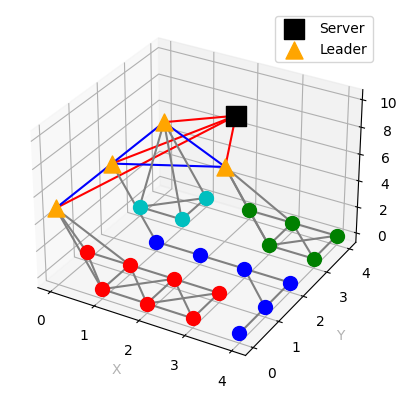
\includegraphics[width=0.5\linewidth]{images/setup/Esempio_Grafo_G.png}
    \caption{Esempio di grafo $G$ con struttura a cluster e overlay tra i leader. Nel livello pi\`u basso sono presenti i nodi normali, disposti su una griglia 5x5 e colorati in base al cluster di appartenenza. Ogni cluster ha un leader, rappresentato da un triangolo arancione, elevato ad un livello superiore. I leader comunicano tra loro attraverso un overlay, mostrato con archi blu, e sono collegati al nodo server, rappresentato da un quadrato nero, mediante archi rossi.}
    \label{fig:enter-label}
\end{figure}

\end{itemize}

\paragraph{Complessit\`a della fase di setup}

Di seguito viene riportata l'analisi della complessit\`a delle due fasi.

\begin{itemize}
    \item \textbf{Fase 1: Formazione dei cluster tramite BFS}
    \begin{itemize}
        \item Il server avvia una BFS per formare i cluster, scorrendo l'immagine da sinistra a destra e dall'alto verso il basso.
        \item Per ogni nodo non ancora visitato, viene avviata una BFS che include tutti i nodi adiacenti con lo stesso colore.
        \item La complessit\`a della BFS per ogni cluster \`e lineare rispetto al numero di nodi nel cluster, ossia $O(k)$, dove $k$ \`e il numero di nodi del cluster.
        \item Poiché ogni nodo dell'immagine viene visitato esattamente una volta, la complessit\`a totale della formazione dei cluster \`e $O(N \times M)$, dove $N \times M$ rappresenta il numero totale di nodi nell'immagine.
    \end{itemize}

    \item \textbf{Fase 2: Scoperta dei cluster adiacenti}
    \begin{itemize}
        \item Dopo la formazione dei cluster, i leader inviano richieste ai propri nodi per verificare se i loro vicini appartengono a un altro cluster.
        \item Ogni nodo comunica solo con i suoi vicini immediati, il che implica una complessit\`a costante per ogni nodo, pari a $O(1)$.
        \item La complessit\`a totale della scoperta dei cluster adiacenti \`e anch'essa $O(N \times M)$, poiché ogni nodo partecipa al processo una sola volta.
    \end{itemize}
    \newpage
    \item \textbf{Rete overlay e sincronizzazione finale}
    \begin{itemize}
        \item Una volta scoperti i cluster adiacenti, viene costruita una rete overlay tra i leader.
        \item Ogni leader comunica con il server e con i leader dei cluster adiacenti.
        \item La complessit\`a di questa fase \`e proporzionale al numero di cluster, ossia $O(C)$, dove $C$ \`e il numero totale di cluster.
    \end{itemize}

    \item \textbf{Conclusione sulla complessit\`a}
    \begin{itemize}
        \item La complessit\`a totale della fase di setup \`e dominata dal numero di nodi nell'immagine, quindi \`e $O(N \times M)$.
        \item Questa complessit\`a si mantiene per la formazione dei cluster tramite BFS e la scoperta dei cluster adiacenti.
        \item Sebbene la costruzione della rete overlay abbia una complessit\`a aggiuntiva $O(C)$, essa \`e limitata rispetto al termine dominante $O(N \times M)$.
        \item Pertanto, la fase di setup risulta essere efficiente e scalabile, anche per immagini di grandi dimensioni.
    \end{itemize}
\end{itemize}

\subsection{Architettura del sistema}

\subsubsection{Nodi}
Il sistema \`e composto da due tipi principali di nodi:

\begin{enumerate}
    \item \textbf{Nodi normali}: rappresentano i pixel dell'immagine e mantengono informazioni minime. Ogni nodo normale conosce:
    \begin{itemize}
        \item Le proprie coordinate \texttt{(x, y)} all'interno dell'immagine.
        \item Il proprio \texttt{leaderID}, che identifica il leader del cluster a cui appartiene.
    \end{itemize}

    \item \textbf{Nodi leader}: sono responsabili della gestione del cluster. Ogni nodo leader mantiene:
    \begin{itemize}
        \item Le proprie coordinate \texttt{(x, y)} all'interno dell'immagine.
        \item Il colore del cluster (\texttt{color}).
        \item La \texttt{lista dei nodi leader} dei cluster adiacenti nel grafo overlay.
        \item L'identificatore del server (\texttt{serverID}).
        \item L'ultimo evento che il nodo ha gestito e il suo rispettivo timestamp (serve per gestire i casi di concorrenza).
        \item La lista \texttt{cluster\_nodes}, ossia i nodi del cluster di cui il leader \`e collegato direttamente.
    \end{itemize}
\end{enumerate}

\subsubsection{Server condiviso} 
Il sistema utilizza un server condiviso per garantire la consistenza globale e sincronizzare le operazioni tra i leader dei cluster. Il server mantiene due strutture chiave: il \textbf{file di log} e lo \textbf{stato globale dei cluster}, entrambe cruciali per il corretto funzionamento e coordinamento del sistema.

\begin{enumerate}
    \item \textbf{File di log}: un registro cronologico delle operazioni eseguite nel sistema, che include informazioni dettagliate su ogni azione eseguita. Ogni operazione nel file di log \`e composta dai seguenti elementi:
    \begin{itemize}
        \item \textbf{Timestamp}: Il momento in cui l'operazione \`e stata eseguita, usato per ordinare temporalmente le azioni.
        \item \textbf{Azione eseguita}: Il tipo di operazione effettuata, come \texttt{merge} (fusione di due cluster), \texttt{color} (cambio di colore di un cluster), ecc.
        \item \textbf{Nodi leader coinvolti}: La lista dei \texttt{leaderID} dei nodi leader che hanno partecipato all'operazione.
        \item \textbf{Nuovo colore}: Il colore finale del cluster, utile nel caso di operazioni di cambio colore o merge. In caso di un'operazione \texttt{merge}, il nuovo colore sar\`a lo stesso dei cluster di partenza.
    \end{itemize}
    \vspace{-20pt}
    \begin{figure}[H]
        \begin{align*}
            &\{ \\
            &\quad \text{(timestamp, azione, [leaderID\_1, leaderID\_2, \ldots], colore)},\\
            &\quad \ldots\\
            &\}
        \end{align*}
        \vspace{-20pt}
        \caption{Struttura del file di log}
    \end{figure}

    \item \textbf{Stato globale dei cluster}: Una matrice che rappresenta lo stato corrente di tutti i cluster nel sistema. Questa struttura consente al server di tenere traccia dello stato attuale e permette di gestire richieste e operazioni con efficienza. Per ogni leader, vengono mantenute le seguenti informazioni:
    \begin{itemize}
        \item \textbf{Identificatore del leader} (\texttt{leaderID}): Un ID univoco che identifica il leader di un cluster.
        \item \textbf{Nodi nel cluster}: La lista completa dei nodi che appartengono al cluster guidato dal leader.
        \item \textbf{Colore attuale del cluster} (\texttt{color}): Il colore corrente assegnato a tutti i nodi del cluster.
        \item \textbf{Cluster adiacenti}: La lista dei leader dei cluster adiacenti nel grafo overlay, che permette ai leader di comunicare tra loro e coordinare operazioni come il merge.
    \end{itemize}
    \vspace{-20pt}
    \begin{figure}[H]
    \begin{align*}
            &\{ \\
            &\ \text{(leaderID, [nodo\_1, nodo\_2, \ldots], colore, [leaderID\_adiacente\_1, leaderID\_adiacente\_2, \ldots])}, \\
            &\ \ldots \\
            &\}
        \end{align*}
        \vspace{-20pt}
        \caption{Struttura dello stato globale dei cluster}
        \label{fig:global_cluster_state}
    \end{figure}

\end{enumerate}

\subsection{Descrizione degli algoritmi}

In questa sezione vengono descritti gli algoritmi chiave utilizzati nel sistema.

\subsubsection{1. Algoritmo di scambio messaggi}
\label{sec:change_colore}
In questa sezione descriviamo gli algoritmi utilizzati in ciascuna fase di scambio messaggi tra nodi interni e leader.

\paragraph{Algoritmo di inizializzazione richiesta}

Ogni nodo hai vari tipi di richieste che pu\`o inoltrare al leader (\ref{sec:tipi_di_messaggi}). Nel seguente pseudo-codice viene preso ad esempio il caso di richiesta di cambio colore da parte di un nodo (\texttt{colorChangeRequest}).

Il nodo scelto inizializza una richiesta di cambio colore, creando un messaggio con tag \\ \texttt{ChangeColorRequest} assieme ai parametri necessari per la richiesta (\texttt{colore} e \texttt{timestamp}) da far recapitare al leader. Il nodo inoltra la richiesta verso il leader tramite il nodo parent.

\begin{algorithm}[H]
\caption{Inizializzazione richiesta di cambio colore}
\begin{algorithmic}[1]
\Procedure{InitChangeColorRequest}{$newColor$}
    \State $msg \gets$ ($node.timestamp$, `colorChangeRequest', $newColor$);
    \State $tries \gets 0$;
    \Do
        \State $response \gets$ await send($node.parent, msg$);
        \State $tries \gets tries + 1$
    \DoWhile{not $response$ and $tries <= 3$}
\EndProcedure
\end{algorithmic}
\end{algorithm}

\paragraph{Algoritmo per l'inoltro delle richieste}

Quando un nodo interno non leader riceve un messaggio, il suo compito \`e semplicemente quello di rispondere al mittente con un ACK ed inoltrare il messaggio al proprio parent. Questo meccanismo di inoltro garantisce che la richiesta raggiunga il leader, passando attraverso tutti i nodi parent nella catena di comunicazione.

\begin{algorithm}[H]
\caption{Inoltro messaggio verso il leader}
\begin{algorithmic}[1]
\Procedure{forwardRequest}{$msg$}
    \State send($msg.sender$, ACK)
    \State $tries \gets 0$;
    \Do
        \State $response \gets$ await send($node.parent, msg$);
        \State $tries \gets tries + 1$
    \DoWhile{not $response$ and $tries <= 3$}
\EndProcedure
\end{algorithmic}
\end{algorithm}

\newpage
\paragraph{1.3 Algoritmo di gestione richieste del leader}

Il leader del cluster pu\`o ricevere vari tipi di richieste (tra cui quella di cambio colore): ciascuna richiesta viene inoltrata al server, il quale si occuper\`a di gestire casi particolari di concorrenza e di memorizzare l'operazione per la ridondanza.

\begin{algorithm}[H]
\caption{Gestione delle richieste nodo leader}
\begin{algorithmic}[1]
\Procedure{leaderReceiveRequest}{$msg$}
    \State $timestamp \gets msg[0]$;
    \State $lastTimestamp \gets log[-1]['timestamp']$;
    \If{$timestamp > lastTimestamp$}
        \State $response \gets$ await send($serverId$, msg);
        \If{$response$}
            \State $requestType \gets msg[1]$;
            \If{$requestType$ == `changeColorRequest'}
                \State $node.color = msg[2]$;
                \State checkMerge();
            \Else
                \State $\ldots$ \Comment{Altri tipi di richieste}
            \EndIf
        \EndIf
        \State sync($log$);
        \State sync($global\_state$);
    \EndIf
\EndProcedure
\end{algorithmic}
\end{algorithm}

Il leader confronta il timestamp del messaggio con quello dell'ultima operazione eseguita salvata nel file di log. Se il timestamp del messaggio \`e pi\`u recente, il leader notifica il server dell'operazione ed in seguito la esegue. La nuova operazione viene registrata nel file di log del server e lo stato globale del cluster viene aggiornato. Nel caso di un'operazione di cambio colore, il leader si occupa di controllare se eseguire un merge o meno in base al colore dei cluster adiacenti.

\subsubsection{2. Algoritmo di merge di cluster}
\label{sec:merge}
Il merge tra due cluster adiacenti viene attivato quando il leader di uno dei cluster effettua un cambio di colore e scopre che il cluster adiacente ha lo stesso colore. Il leader che ha avviato il cambio colore invia la richiesta di merge al leader del cluster adiacente, indipendentemente dagli ID dei leader.

\newpage
\paragraph{Situazione 1: richiesta di merge da leader con ID maggiore a uno con ID minore}
In questo scenario, il leader con ID maggiore invia una richiesta di merge al leader del cluster con ID minore. Il leader con ID minore accetta la richiesta, e il leader con ID maggiore si trasforma in un nodo normale. 

\vspace{-5pt}
\begin{algorithm}[H]
\caption{Richiesta di merge da leader con ID maggiore}
\begin{algorithmic}[1]
\Procedure{InvioMergeDaIDMaggiore}{$leaderIDMinore$}
    \State $response \gets$ await send($leaderIDMinore$, `mergeRequest');
    \If{$response$}
        \State $msg$ = (`leaderUpdate', $leaderIDMinore$);
        \For{$child$ in $node.children$}
            \State send($child$, $msg$);
        \EndFor      
        \State $node.parent \gets leaderIDMinore$;
        \State $node.type \gets$ `node';
        \State send($leaderIDMinore$, $node.adjList$);
        \State send($leaderIDMinore$, `ackMergeCompletato');
    \EndIf
\EndProcedure
\end{algorithmic}
\end{algorithm}

\vspace{-15pt}
\begin{algorithm}[H]
\caption{Ricezione richiesta di merge al leader con ID minore}
\begin{algorithmic}[1]
\Procedure{RicezioneMergeDaIDMaggiore}{$leaderIDMaggiore$, $request$}
    \If{$request$ == `mergeRequest'}
        \State send($leaderIDMaggiore$, ACK);
        \State $adjListIDMaggiore \gets$ receive();
        \State $node.adjList \gets$ join($node.adjList, adjListIDMaggiore$);
    \EndIf
\EndProcedure
\end{algorithmic}
\end{algorithm}

\vspace{-10pt}
\begin{figure}[H]
    \centering
    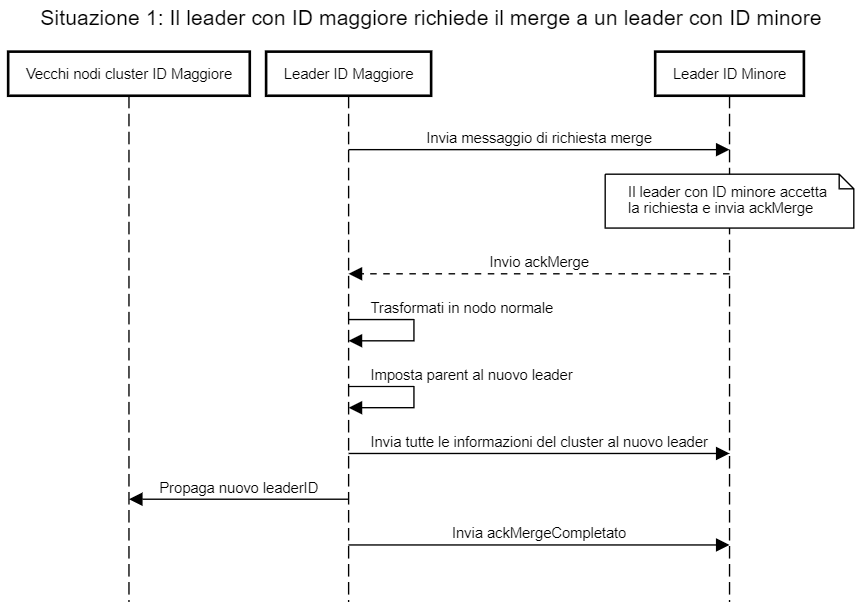
\includegraphics[width=0.85\linewidth]{images/Situazione1.png}
    % \caption{Diagramma della Situazione 1}
\end{figure}

\paragraph{Situazione 2: richiesta di merge da leader con ID minore a uno con ID maggiore}
Questo scenario \`e contrapposto al precedente presentato in quanto \`e il leader con ID minore ad inviare una richiesta di merge ad un leader adiacente con ID maggiore. Il leader con ID maggiore accetta la richiesta e si trasforma in un nodo normale.

\vspace{-5pt}
\begin{algorithm}[H]
\caption{Richiesta di merge da leader con ID minore}
\begin{algorithmic}[1]
\Procedure{InvioMergeDaIDMinore}{$leaderIDMaggiore$}
    \State $response \gets$ await send($leaderIDMaggiore$, `mergeRequest');
    \If{$response$}
        \State send($leaderIDMaggiore$, ACK);
        \State $adjListIDMaggiore \gets$ receive();
        \State $node.adjList \gets$ join($node.adjList, adjListIDMaggiore$);
    \EndIf
\EndProcedure
\end{algorithmic}
\end{algorithm}

\vspace{-15pt}

\begin{algorithm}[H]
\caption{Ricezione richiesta di merge al leader con ID maggiore}
\begin{algorithmic}[1]
\Procedure{RicezioneMergeDaIDMinore}{$leaderIDMinore$, $request$}
    \If{$request$ == `mergeRequest'}
        \State $msg$ = (`leaderUpdate', $leaderIDMinore$);
        \For{$child$ in $node.children$}
            \State send($child$, $msg$);
        \EndFor
        \State $node.parent \gets leaderIDMinore$;
        \State $node.type \gets$ `node';
        \State send($leaderIDMinore$, $node.adjList$);
        \State send($leaderIDMinore$, `ackMergeCompletato');
    \EndIf
\EndProcedure
\end{algorithmic}
\end{algorithm}

\vspace{-20pt}
\begin{figure}[H]
    \centering
    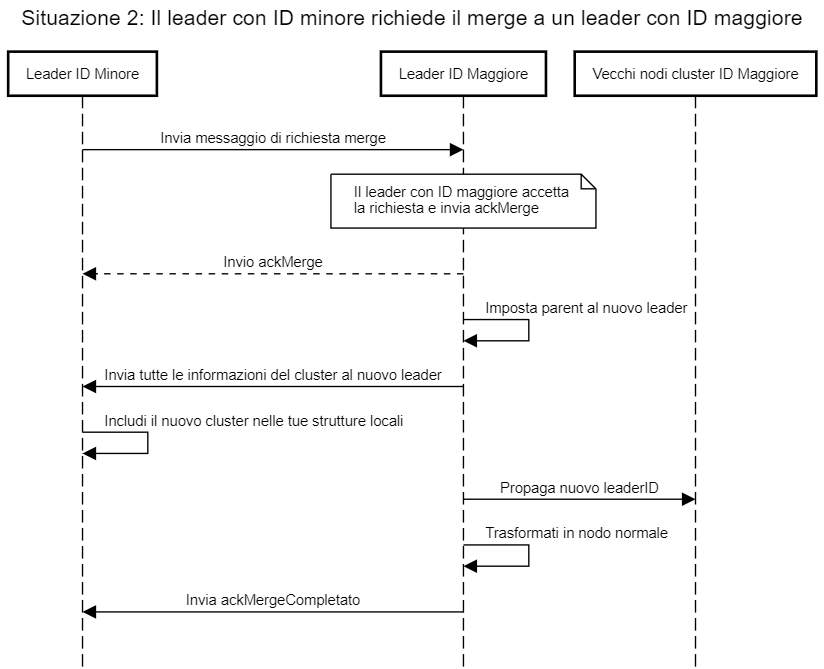
\includegraphics[width=0.75\linewidth]{images/Situazione2.png}
    % \caption{Diagramma della Situazione 2}
\end{figure}

\subsection{Gestione dei messaggi e della comunicazione}\label{sec:gestione_messaggi}

La comunicazione tra i nodi \`e un aspetto fondamentale per il corretto funzionamento del sistema distribuito, specialmente in un contesto di sincronizzazione e consistenza. Di seguito vengono analizzati i tipi di messaggi utilizzati, il protocollo di comunicazione e la gestione di eventuali ritardi o fallimenti.

\subsubsection{Tipi di messaggi}
\label{sec:tipi_di_messaggi}

Nel sistema sono utilizzati diversi tipi di messaggi per coordinare le operazioni, sia tra i nodi normali che tra i leader e il server centrale:

\begin{itemize}
    \item \textbf{Messaggi di propagazione dell'ID leader}: utilizzati durante la formazione e la gestione dei cluster, questi messaggi servono a diffondere l'\texttt{id\_leader} ai nodi appartenenti al cluster, assicurando che tutti conoscano il proprio leader.
    \item \textbf{Richieste di cambio colore (\texttt{colorChangeRequest})}: inviate dai nodi normali verso il leader del proprio cluster quando desiderano avviare un'operazione di cambio colore. Questi messaggi contengono le informazioni sul nuovo colore e sul timestamp dell'operazione(vedi sezione \ref{sec:change_colore}).
    \item \textbf{Messaggi di conferma (ACK)}: utilizzati per garantire l'affidabilit\`a del sistema, questi messaggi confermano la corretta ricezione delle richieste critiche. In caso di mancata risposta, viene ritentato l'invio (per una spiegazione pi\`u dettagliata \ref{sec:ack}).
    \item \textbf{Messaggi di merge (\texttt{mergeRequest})}: scambiati tra i leader di cluster adiacenti durante le operazioni di unione dei cluster. Dopo la richiesta di merge, il leader che accetta l'operazione invia un \texttt{ackMerge} per confermare l'unione (vedi sezione \ref{sec:merge}).
    \item \textbf{Messaggi di \texttt{heartbeat}}: inviati periodicamente tra le varie componenti del sistema, servono per monitorare la disponibilit\`a e la salute dei nodi (normali e leader), e rilevare eventuali fallimenti (per una spiegazione dettagliata \ref{sec:fallimento_leader}). 
    \item \textbf{Messaggi al server}: i nodi leader comunicano con il server per aggiornare lo stato globale del cluster, registrare le operazioni nel file di log, e segnalare eventuali fusioni, cambi di colore o fallimenti.
    \item \textbf{Messaggi di BFS\_Request}: utilizzato durante la fase di riconfigurazione in caso di fallimento di un nodo, questo messaggio viene inviato da un nodo figlio verso i suoi vicini quando tenta di ristabilire la connettivit\`a con il leader o altri nodi del cluster. Il messaggio contiene il \texttt{leaderID} del nodo che ha avviato la ricerca e viene propagato fino a quando non si trova un nodo connesso al leader (per una spiegazione dettagliata \ref{sec:fallimento_nodo_normale}). 
\end{itemize}

\newpage
\subsubsection{Protocollo di comunicazione}
\label{sec:ack}
Per garantire un alto grado di affidabilit\`a e tolleranza ai guasti, il sistema implementa un protocollo basato su conferme (ACK) e ritrasmissioni in caso di timeout:

\begin{itemize}
    \item \textbf{Invio del messaggio}: ogni volta che un nodo invia un messaggio critico (es. richiesta di cambio colore o \texttt{mergeRequest}), avvia un timer di timeout.
    \item \textbf{Conferma di ricezione (ACK)}: il nodo ricevente, dopo aver elaborato il messaggio, invia un \texttt{ACK} al mittente per confermare la corretta ricezione e processazione.
    \item \textbf{Ritrasmissione in caso di timeout}: se il mittente non riceve l'\texttt{ACK} entro un tempo predefinito, ritrasmette il messaggio. Viene eseguito un numero massimo di ritrasmissioni prima che il nodo consideri il destinatario come non raggiungibile.
    \item \textbf{Numero massimo di tentativi}: se un nodo non riceve conferma dopo un certo numero di tentativi, considera il nodo destinatario come fallito e inizia le procedure di recupero.
\end{itemize}

\subsubsection{Gestione dei ritardi e dei messaggi fuori ordine}

Considerando che i messaggi in rete possono subire ritardi e arrivare fuori ordine, il sistema utilizza meccanismi di controllo dei timestamp e gestione delle operazioni per evitare incongruenze:

\begin{itemize}
    \item \textbf{Timestamp e identificatori univoci}: ogni messaggio \`e accompagnato da un timestamp e un identificatore univoco per garantire che sia elaborato correttamente e nell'ordine appropriato. I nodi utilizzano questi dati per determinare l'ordine delle operazioni.
    \item \textbf{Gestione dei messaggi duplicati}: il sistema ignora automaticamente i messaggi duplicati (ossia gi\`a ricevuti ed elaborati), riducendo l'overhead di calcolo e prevenendo errori di consistenza.
    \item \textbf{Ordinamento delle operazioni}: nel caso di ricezione di messaggi fuori ordine, il sistema applica le operazioni basandosi sui timestamp per garantire che vengano eseguite nel corretto ordine temporale.
\end{itemize}
\newpage
\subsection{Gestione dei timestamp} \label{sec
}

Per garantire un ordinamento coerente degli eventi e mantenere la consistenza causale, \`e stato scelto di aggiungere al sistema distribuito un server per il tempo centralizzato.

L'impiego dei timestamp risulta fondamentale per la gestione sia delle richieste di cambio colore che di quelle di merge, poiché, per risolvere casi di concorrenza, viene fatto un ordinamento delle operazioni basato sul tempo di invio della richiesta. L'ordinamento permette sia di gestire in maniera precisa le possibili situazioni di concorrenza affrontate nella sezione \ref{sec
}, sia di registrare le operazioni in un unico file di log.

\paragraph{Utilizzo nel sistema}

Il sistema prevede che il time-server invii periodicamente i timestamp aggiornati a ciascun nodo, riducendo così il sovraccarico di richieste al time-server. Ogni nodo memorizza un timestamp locale, che viene aggiornato con i dati ricevuti dal time-server. Questo approccio garantisce che i timestamp dei nodi siano sincronizzati senza la necessit\`a di contattare continuamente il server, evitando così di sovraccaricare il sistema con troppe richieste.

\paragraph{Risoluzione dei conflitti}

In caso di conflitti tra operazioni concorrenti (ad esempio, due richieste ricevute quasi simultaneamente), l'operazione con il timestamp minore ha la precedenza. In caso di parit\`a di timestamp, si pu\`o utilizzare un criterio di tie-breaker, come l'ID del nodo mittente.

\paragraph{Considerazioni sulla scelta}

\`e stato preso in considerazione anche l'utilizzo di un orologio logico, in particolare quello proposto da Lamport. Tuttavia, data sia la struttura di rete, sia la direzione dei messaggi trasmessi (convergente verso il leader), l'utilizzo di timestamp aggiornati tramite un time-server centrale risulta pi\`u efficiente in termini di performance e numero di messaggi scambiati. L'implementazione dell'orologio logico di Lamport richiederebbe un continuo scambio di messaggi tra i nodi per mantenere i timestamp locali sincronizzati, con un overhead significativo.

Come descritto nel dettaglio nella precedente sezione \ref{sec
} sulla comunicazione, ogni richiesta confluisce verso il leader e il sistema di request-response basato su ACK \`e implementato unicamente tra due nodi direttamente comunicanti. L'utilizzo dell'orologio logico di Lamport, senza l'aggiunta di messaggi di risposta in direzione contraria, causerebbe col tempo un disallineamento tra i timestamp dei nodi meno attivi e quelli del leader, rendendo le loro richieste sempre pi\`u obsolete e infine scartate.

Inoltre, l'orologio logico di Lamport risulterebbe problematico per un ordinamento globale delle operazioni all'interno del log, poiché ogni cluster sarebbe temporalmente indipendente dagli altri, legato al numero di richieste ricevute dal proprio leader.

\paragraph{Limitazioni dell'approccio}

Nonostante i vantaggi, questo approccio presenta la criticit\`a di introdurre un singolo punto di fallimento nel sistema: il time-server centrale. Se il time-server dovesse fallire o diventare non raggiungibile, gli orologi dei nodi non verrebbero pi\`u sincronizzati con esso, creando il rischio di presentare divergenze tra gli orologi dei nodi, i quali causerebbero possibili inconsistenze nell'ordinamento delle operazioni. Questo problema potrebbe compromettere la correttezza del sistema e richiedere meccanismi di tolleranza ai guasti o la presenza di server di tempo ridondanti per garantire la continuit\`a del servizio.

\newpage
\subsection{Gestione della consistenza}\label{sec:gestione_consistenza}

Per garantire la consistenza del sistema, vengono gestiti tre casi principali:

\paragraph{Caso 1: Richiesta di cambio colore con timestamp anteriore che richiede un merge}

Se dopo un'operazione di cambio colore con timestamp $T_2$, arriva una richiesta con timestamp $T_1 < T_2$ che avrebbe generato un merge con un cluster adiacente all'epoca $T_1$ (figura \ref{fig:caso1_concorrenza}):

\begin{itemize}
    \item Si eseguono operazioni di ripristino per riportare lo stato al tempo $T_1$.
    \item Si esegue il merge tra i due cluster.
    \item Si applica il nuovo colore risultante dall'operazione pi\`u recente.
\end{itemize}

\begin{figure}[H]
    \centering
    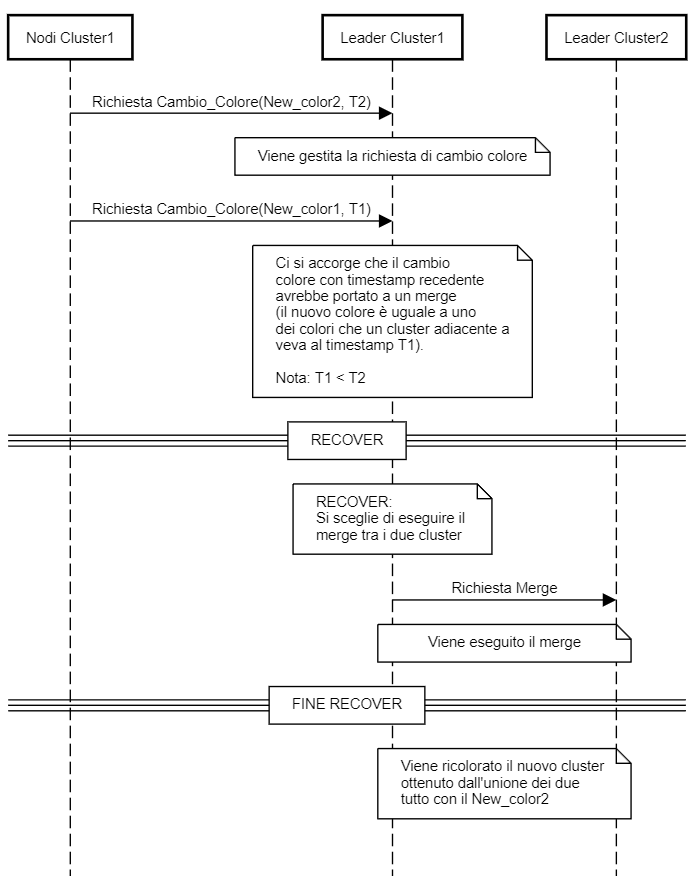
\includegraphics[width=0.65\textwidth,align=t]{images/concorrenza/caso1.png}
    \caption{Caso 1: Richiesta di cambio colore con timestamp anteriore che richiede un merge}
    \label{fig:caso1_concorrenza}
\end{figure}

\newpage
\paragraph{Caso 2: Richiesta di cambio colore con timestamp anteriore che non richiede un merge}

Se la richiesta con timestamp $T_1 < T_2$ non avrebbe generato un merge all'epoca $T_1$, ma l'operazione successiva con $T_2$ ha gi\`a effettuato un merge (figura \ref{fig:caso2_concorrenza}):

\begin{itemize}
    \item Si ignora l'azione con timestamp $T_1$ poiché lo stato attuale non corrisponde pi\`u alle condizioni dell'epoca $T_1$.
\end{itemize}

\begin{figure}[H]
    \centering
    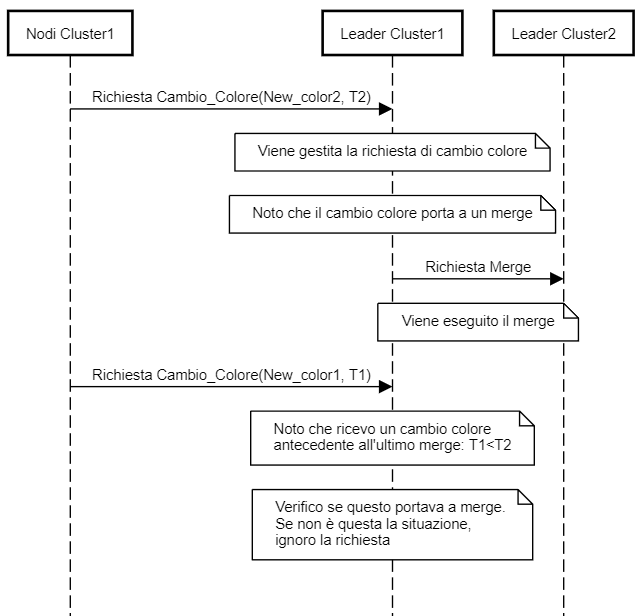
\includegraphics[width=0.65\textwidth,align=t]{images/concorrenza/caso2.png}
    \caption{Caso 2: Richiesta di cambio colore con timestamp anteriore che non richiede un merge}
    \label{fig:caso2_concorrenza}
\end{figure}

\newpage
\paragraph{Caso 3: Richiesta di merge ricevuta mentre \`e in corso un cambio colore con timestamp anteriore}

Quando un leader riceve una richiesta di merge ma \`e in attesa di una richiesta di cambio colore con timestamp anteriore (figura \ref{fig:caso3_concorrenza}):

\begin{itemize}
    \item Il leader attende per un periodo di tempo sufficiente per ricevere eventuali richieste in ritardo.
    \item Se dopo il timeout non arrivano nuove richieste, procede con il merge.
    \item Questo approccio previene inconsistenze dovute a operazioni fuori ordine.
\end{itemize}

\begin{figure}[H]
    \centering
    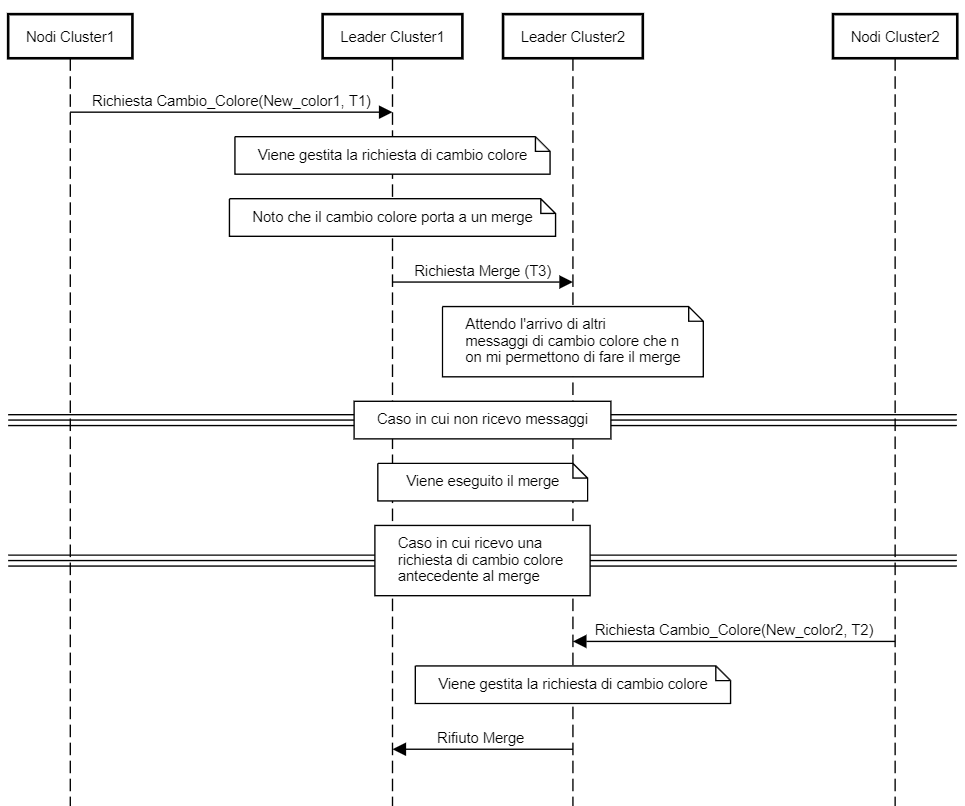
\includegraphics[width=0.65\textwidth,align=t]{images/concorrenza/caso3.png}
    \caption{Caso 3: Richiesta di merge ricevuta mentre \`e in corso un cambio colore con timestamp anteriore}
    \label{fig:caso3_concorrenza}
\end{figure}

\subsection{Gestione dei fallimenti}

La robustezza del sistema dipende dalla capacit\`a di gestire efficacemente i fallimenti dei nodi, sia leader che normali. Di seguito vengono dettagliate le strategie adottate per ricalcolare la struttura del cluster in caso di fallimenti, con particolare attenzione ai casi limite.

\subsubsection{1. Fallimento di un nodo leader}
\label{sec:fallimento_leader}
Il leader di un cluster \`e fondamentale per la coordinazione e la comunicazione all'interno del cluster stesso. Tuttavia, il fallimento di un leader pu\`o generare scenari complessi, come la formazione di sotto-grafi disconnessi. Il sistema deve quindi gestire efficacemente tali situazioni per garantire la continuit\`a operativa e la coerenza del cluster.

\begin{itemize}
    \item \textbf{Monitoraggio tramite heartbeat:} I leader e il server scambiano continuamente messaggi di \texttt{heartbeat} per monitorare lo stato di salute dei leader.
    \item \textbf{Rilevamento del fallimento:} Se il server o un altro leader non riceve un \texttt{heartbeat} da un leader entro un tempo prefissato (\textit{timeout}), assume che il leader sia fallito.
    \item \textbf{Gestione del partizionamento in sotto-grafi:}
    \begin{itemize}
        \item Quando un leader fallisce, il server elegge il nodo con l'\texttt{id} pi\`u basso rimasto e lo nomina come nuovo leader. 
        \item Il nuovo leader avvia una BFS per ristabilire la struttura gerarchica del suo sotto-grafo e comunica al server i nodi che fanno parte del sotto-grafo rimanente.
        \item Il server controlla se ci sono nodi non inclusi nel nuovo sotto-grafo e, per ogni gruppo di nodi sconnessi, elegge altri nuovi leader per gestire i restanti sotto-grafi.
        \item Il processo continua finché tutti i nodi disconnessi non vengono riassegnati a un leader e il cluster non \`e completamente ripristinato.
    \end{itemize}
    \item \textbf{Ricostruzione della struttura del cluster:}
    \begin{itemize}
        \item Durante la BFS, ogni nodo del sotto-grafo riassegnato aggiorna il proprio \texttt{leaderID} con quello del nuovo leader.
        \item Vengono sistemate le relazioni di \texttt{parent} e \texttt{child} tra i nodi per garantire la connessione all'interno del sotto-grafo.
        \item Vengono comunicati eventuali cluster adiacenti al nuovo leader in modo che possa aggiornare la rete overlay.
    \end{itemize}
\end{itemize}

\textbf{Casi limite da gestire:}

\begin{itemize}
    \item \textit{Partizionamento in pi\`u sotto-grafi disconnessi:} Se il fallimento del leader causa la formazione di pi\`u sotto-grafi disconnessi, il server si assicura che ogni sotto-grafo venga gestito in modo indipendente con un nuovo leader. Il processo continua fino a quando tutti i nodi del cluster originario non sono stati riassegnati.
    \item \textit{Inconsistenze durante l'elezione:} Per evitare condizioni di competizione (\textit{race conditions}), i nodi seguono una politica deterministica basata sull'\texttt{id} pi\`u basso per eleggere il nuovo leader in ciascun sotto-grafo.
\end{itemize}

\subsubsection{2. Fallimento di un nodo normale}
\label{sec:fallimento_nodo_normale}
Il fallimento di un nodo non leader pu\`o avere impatti diversi sulla struttura del cluster, a seconda del ruolo del nodo e della sua posizione all'interno dell'albero di comunicazione.

\begin{itemize}
    \item \textbf{Nodo foglia:} Se il nodo fallito \`e una foglia, il suo fallimento non interrompe la comunicazione tra gli altri nodi del cluster. Nessuna azione \`e necessaria.
    
    \item \textbf{Nodo interno:} Se il nodo \`e interno e il suo fallimento interrompe la comunicazione tra parti del cluster, \`e necessario ricalcolare la struttura per ristabilire la connettivit\`a. Questo processo coinvolge diverse fasi dettagliate di seguito.

    \newpage
    \begin{enumerate}
        \item \textbf{Rilevamento del fallimento:}
        \begin{itemize}
            \item \textbf{Tentativi di comunicazione:} Il nodo figlio del nodo fallito tenta di comunicare con il proprio \texttt{parent} per operazioni periodiche (ad esempio, messaggi di \texttt{heartbeat}) o in risposta a eventi specifici (come richieste di cambio colore).
            \item \textbf{Timeout e assunzione di fallimento:} Se il nodo figlio non riceve risposta dopo un certo numero di tentativi, utilizzando meccanismi di \texttt{ack} (acknowledgment) e un intervallo di \textit{timeout}, assume che il \texttt{parent} sia fallito.
        \end{itemize}
        
        \item \textbf{Inizio della prima BFS (riconfigurazione):}
        \begin{itemize}
            \item \textbf{Avvio di una BFS locale:} Il nodo figlio avvia una \textit{Breadth-First Search} (BFS) per esplorare i nodi raggiungibili con lo stesso \texttt{leaderID}, inviando messaggi di \texttt{BFS\_Request} ai propri vicini. L'obiettivo \`e capire se esiste un percorso alternativo per raggiungere il leader originale.
            \item \textbf{Tracciamento delle richieste:} Durante la BFS, ogni nodo che riceve un \texttt{BFS\_Request} si segna da quale nodo \`e arrivata la richiesta, così da poter ripercorrere all'indietro il percorso seguito dalla richiesta una volta trovato un nodo connesso al leader.
        \end{itemize}
        
        \item \textbf{Analisi dei risultati della prima BFS:}
        \begin{enumerate}
            \item \textbf{Caso 1 - Cluster non isolato (leader raggiungibile):}
            Se la BFS raggiunge il leader originale il percorso seguito dalla prima BFS viene ripercorso all'indietro, aggiornando solo i nodi coinvolti direttamente nella ricostruzione del percorso e ristabilendo la connessione al nodo sconnesso aggiornando i \texttt{parent} dei nodi.

            \item \textbf{Caso 2 - Cluster isolato (leader non raggiungibile):}
            Se la BFS non trova alcun percorso per raggiungere il leader originale, significa che il sotto-grafo \`e diventato isolato dal cluster principale. Il nodo che ha avviato la BFS attende prima di avviare altre azioni:
            \begin{itemize}
                \item \textbf{Attesa delle risposte:} Il nodo attende di ricevere risposte da tutti i nodi raggiunti dalla BFS. Se nessuno dei nodi risponde di essere collegato al leader, il nodo si autoproclama leader.
                \item \textbf{Avvio della seconda BFS (nuovo leader):} Una volta autoproclamato leader, il nodo avvia una seconda BFS per informare tutti i nodi del sotto-grafo che \`e diventato il nuovo leader.
                \item \textbf{Aggiornamento dei nodi:} Tutti i nodi raggiunti dalla BFS aggiornano il proprio \texttt{leaderID} con quello del nuovo leader.
                \item \textbf{Comunicazione al server:} Il nuovo leader invia un messaggio di \\ \texttt{NewLeaderAnnouncement} al server, informandolo della formazione del nuovo cluster e fornendo la lista dei nodi coinvolti.
            \end{itemize}
        \end{enumerate}
    \end{enumerate}
\end{itemize}

\subsection{Criteri di selezione del leader}

In un sistema distribuito come quello descritto, la selezione di un leader all'interno di un cluster di nodi \`e fondamentale per garantire efficienza operativa e tolleranza ai guasti. Nel contesto dell'algoritmo Flood-Fill distribuito, dove ogni nodo rappresenta un pixel, i leader devono essere scelti in modo da minimizzare la complessit\`a e garantire la robustezza. Di seguito, vengono discussi i criteri utilizzati per la selezione del leader.

\subsubsection{Attribuzione dell'ID ai nodi}

Ogni nodo nel sistema rappresenta un pixel di una matrice bidimensionale, e a ciascun nodo viene assegnato un identificatore unico (ID). Per generare l'ID dei nodi, si utilizzano le coordinate del pixel \texttt{(x, y)} all'interno della matrice. Esistono diversi metodi per attribuire un ID:

\begin{itemize}
    \item \textbf{Utilizzo delle coordinate \texttt{(x, y)}}: Le coordinate stesse possono essere utilizzate come identificatore. In questo caso, l'ID del nodo sar\`a la coppia \texttt{(x, y)}, che rappresenta la posizione esatta del nodo nella matrice.
    
    \item \textbf{Linearizzazione delle coordinate}: Per ottenere un ID scalare unico, \`e possibile convertire le coordinate \texttt{(x, y)} in un unico valore intero utilizzando la seguente formula:
    \[
    ID_{nodo} = y \times larghezza + x
    \]
    dove $larghezza$ \`e il numero di colonne della matrice. Questa rappresentazione permette di gestire pi\`u facilmente i nodi come valori interi unici.

\end{itemize}

Nel sistema descritto, si utilizza la \textbf{linearizzazione delle coordinate} per ottenere un ID univoco per ciascun nodo. Questo approccio garantisce una rappresentazione compatta ed efficiente dei nodi.

\subsubsection{Selezione del leader}

Una volta che a ciascun nodo \`e stato attribuito un ID, \`e necessario un criterio per la selezione del leader all'interno di ciascun cluster. I criteri di selezione possono variare in base alle esigenze del sistema, ma nel contesto di questo progetto si utilizza il seguente approccio:

\paragraph{ID pi\`u basso come leader}
Il criterio principale adottato \`e la selezione del nodo con l'ID pi\`u basso all'interno del cluster. Questo approccio offre diversi vantaggi:
\begin{itemize}
    \item \textbf{Semplicit\`a}: La selezione del leader basata sull'ID pi\`u basso \`e semplice da implementare e non richiede calcoli complessi o monitoraggi continui.
    \item \textbf{Determinismo}: Il nodo con l'ID pi\`u basso \`e sempre determinabile, garantendo che la selezione del leader sia univoca e ripetibile.
\end{itemize}

\paragraph{Failover e rielezione}
Nel caso in cui il leader selezionato fallisca, \`e previsto un meccanismo di failover automatico. I nodi del cluster avviano un'elezione per scegliere un nuovo leader, basata nuovamente sul criterio dell'ID pi\`u basso tra i nodi rimanenti. Questo processo garantisce che il cluster possa continuare a funzionare correttamente anche in presenza di guasti.

\newpage
\subsection{Vantaggi della soluzione proposta}

La soluzione scelta presenta diversi vantaggi:

\begin{itemize}
    \item \textbf{Scalabilit\`a}: trattando i cluster come nodi in un grafo overlay, il sistema pu\`o gestire efficacemente reti di grandi dimensioni.
    \item \textbf{Consistenza globale}: l'uso del database condiviso garantisce la sincronizzazione delle operazioni e la consistenza dello stato globale.
    \item \textbf{Robustezza ai fallimenti}: i meccanismi di gestione dei fallimenti assicurano che il sistema possa recuperare rapidamente da guasti di nodi leader o interni.
    \item \textbf{Efficienza}: la comunicazione \`e ottimizzata utilizzando i nodi leader all'interno dei cluster e il grafo overlay tra i leader.
\end{itemize}

\section{Piano di Sviluppo}

Il piano di sviluppo del sistema \`e organizzato in sei fasi principali, ciascuna mirata a implementare aspetti cruciali del sistema distribuito, iniziando dalle funzionalit\`a di base fino ad arrivare alla gestione di consistenza e fault tolerance. Di seguito, vengono dettagliate le fasi del progetto:

\subsection*{Fase 1: Implementazione della Comunicazione Base e Setup}

La prima fase \`e focalizzata sull'implementazione della comunicazione essenziale tra i nodi e sulla corretta configurazione della rete. L'obiettivo \`e garantire che ogni nodo possa scambiare messaggi con i nodi vicini e che la fase di setup, inclusa l'assegnazione dei leader e la costruzione del grafo dei cluster, funzioni correttamente.

\subsection*{Fase 2: Implementazione dell'Algoritmo di Cambio Colore}

Una volta che la comunicazione base \`e stabilita, viene implementato l'algoritmo di cambio colore. Questo algoritmo permetter\`a a un nodo di avviare l'operazione di ricolorazione che si propagher\`a ai nodi adiacenti dello stesso cluster, sotto il coordinamento del leader.

\subsection*{Fase 3: Implementazione dell'Algoritmo di Merge}

Nella terza fase, viene sviluppato l'algoritmo di merge, che gestisce la fusione di cluster adiacenti quando questi acquisiscono lo stesso colore. L'algoritmo deve garantire che i leader dei cluster coinvolti collaborino per eseguire l'unione in maniera efficiente e consistente.

\subsection*{Fase 4: Implementazione del Server di Gestione del Tempo e Server Centrale}

In questa fase, viene implementato un server centrale che gestisce i timestamp e coordina le operazioni tra i cluster. Il server avr\`a il compito di mantenere una visione globale dello stato del sistema e garantire che gli eventi vengano ordinati correttamente nel tempo, migliorando così la coerenza globale.

\subsection*{Fase 5: Gestione della Consistenza Globale}

Una volta implementato il server centrale, viene sviluppato un sistema di gestione della consistenza globale. Questo sistema garantisce che le operazioni distribuite, come i cambi di colore e i merge, siano ordinate in maniera corretta, evitando conflitti e garantendo che tutti i nodi abbiano una visione coerente dello stato del sistema.

\subsection*{Fase 6: Gestione dei Fallimenti}

Nell'ultima fase, vengono implementati i meccanismi per gestire i fallimenti dei nodi, sia normali che leader. Questo include la rilevazione dei fallimenti, l'elezione di nuovi leader in caso di guasti e la riconfigurazione del sistema per mantenere la continuit\`a operativa anche in presenza di nodi falliti. L'obiettivo \`e garantire che il sistema sia resiliente e possa continuare a funzionare correttamente anche in condizioni di fault.

\section{Conclusioni}

La soluzione proposta, basata sul trattamento dei cluster come nodi in un grafo overlay e sull'uso di un database condiviso per la sincronizzazione, offre un equilibrio tra efficienza, scalabilit\`a e robustezza. I meccanismi di gestione della consistenza e dei fallimenti garantiscono il corretto funzionamento del sistema in ambienti distribuiti e soggetti a guasti.


\newpage

\chapter{Implementazione}

\section{Scelta del linguaggio di programmazione}

Per questo progetto distribuito sono stati utilizzati due linguaggi di programmazione principali: \textbf{Erlang} e \textbf{Python}. Ciascuno di essi è stato scelto per le sue caratteristiche specifiche, che permettono di risolvere efficacemente problemi di distribuzione e visualizzazione.

\subsection{Erlang}

\textbf{Erlang} è stato scelto per la logica distribuita e la gestione dei nodi nel sistema, grazie alla sua robustezza e al supporto nativo per la concorrenza e la tolleranza ai guasti. Erlang è particolarmente adatto per applicazioni distribuite e fault-tolerant, ed è ampiamente utilizzato in ambiti come le telecomunicazioni e i sistemi di backend ad alta disponibilità.

\begin{itemize}
    \item \textbf{Gestione dei processi}: in Erlang, ogni nodo e leader è gestito come un processo indipendente. Questo permette al sistema di scalare facilmente e di mantenere l'isolamento dei fallimenti tra i nodi.
    \item \textbf{Pattern matching e concorrenza}: Erlang utilizza il pattern matching per la gestione dei messaggi e le strutture dati, facilitando la scrittura di codice conciso e mantenibile. La concorrenza è una funzionalità nativa del linguaggio, che permette ai processi di comunicare tramite messaggi in maniera asincrona.
    \item \textbf{Semplicità e resilienza}: Erlang implementa una semplice struttura di error handling in cui, invece di cercare di prevenire ogni possibile errore, i processi possono fallire e riavviarsi autonomamente. Questo modello “let it crash” è efficace in sistemi distribuiti dove i singoli componenti devono rimanere resilienti.
\end{itemize}

Erlang è quindi stato impiegato per la creazione e gestione dei nodi, la comunicazione tra essi e per mantenere il server centrale che coordina i leader e gestisce la propagazione dei messaggi.

\subsection{Python}

\textbf{Python} è stato scelto per la visualizzazione dei dati e l’interfaccia utente. Con la libreria \texttt{Flask}, è stato possibile implementare un server web per mostrare la matrice dei nodi e permettere l'interazione dell'utente, mentre \texttt{Matplotlib} è stato utilizzato per la grafica della griglia.

\begin{itemize}
    \item \textbf{Visualizzazione e interfaccia web}: Python, con \texttt{Flask} e \texttt{Matplotlib}, permette di creare interfacce web e rappresentazioni grafiche dei nodi in modo rapido e flessibile.
    \item \textbf{Aggiornamenti in tempo reale}: Il supporto di \texttt{Flask-SocketIO} consente la comunicazione in tempo reale tra il backend e l'interfaccia utente, permettendo di aggiornare la visualizzazione della griglia dei nodi ogni volta che avvengono modifiche nel sistema.
    \item \textbf{Facilità d'integrazione con Erlang}: Python comunica con Erlang tramite un server TCP implementato in Erlang stesso. Questo approccio rende semplice l'integrazione e il passaggio di messaggi per operazioni come il cambio di colore dei nodi.
\end{itemize}

Python è quindi stato utilizzato come componente di frontend, fornendo una rappresentazione visiva intuitiva e permettendo l'interazione con i nodi per modificarne lo stato in tempo reale.

\subsection{Benefici della combinazione di Erlang e Python}

La combinazione di Erlang e Python ha permesso di sfruttare il meglio di entrambi i linguaggi:
\begin{itemize}
    \item \textbf{Distribuzione e resilienza} con Erlang per la gestione dei nodi e della logica di sistema.
    \item \textbf{Visualizzazione intuitiva e interattiva} con Python per fornire un’interfaccia utente che permette di osservare lo stato del sistema e interagire con esso.
\end{itemize}

Questo approccio ha consentito di mantenere un sistema distribuito robusto e allo stesso tempo di offrire una visualizzazione efficace e flessibile.


\section{Comandi principali per l'avvio del sistema}

Di seguito sono riportati i comandi da utilizzare in una sessione Erlang per compilare i moduli e avviare il sistema distribuito, seguiti dai comandi per lanciare il visualizzatore Python.

\begin{tcolorbox}[title=Comandi di Avvio in Erlang]
\begin{verbatim}
erl 
c(node).
c(event).
c(utils).
c(operation).
c(setup).
c(server).
c(tcp_server).
c(start_system).
start_system:start(10,10,false).
\end{verbatim}
\end{tcolorbox}

Questi comandi eseguono le seguenti operazioni:
\begin{itemize}
    \item \texttt{c(module).} compila il modulo specificato in Erlang.
    \item \texttt{start\_system:start(10,10,false).} avvia il sistema con una griglia di nodi di dimensioni 10x10. Il terzo parametro indica se usare un file con una lista di colori o meno. Nel caso \texttt{false}, i colori vengono scelti randomicamente da una palette.
\end{itemize}

Per avviare la parte di visualizzazione in Python, che consente di'interagire con il sistema tramite un'interfaccia grafica, è necessario eseguire il seguente comando in un'altra sessione terminale:

\begin{tcolorbox}[title=Avvio dell'interfaccia grafica in Python]
\begin{verbatim}
python3 grid_visualizer.py
\end{verbatim}
\end{tcolorbox}

Questo comando esegue il file \texttt{grid\_visualizer.py}, che lancia un server Flask per la visualizzazione della griglia dei nodi e la gestione dell'interfaccia utente. Il server Python si connette al sistema Erlang tramite un'interfaccia TCP, permettendo la comunicazione tra i due ambienti e l'aggiornamento dinamico della visualizzazione. \`E inoltre possibile fornire come opzione \texttt{--debug} per avere dettagli maggiori riguardo i nodi nell'interfaccia.

\section{Records}

Le principali strutture dati utilizzate sono rappresentate dai record `node` e `leader`, che organizzano le informazioni di ciascun nodo e dei leader dei cluster. Questi record sono definiti in \texttt{node.erl} e permettono di gestire la posizione, i vicini e l'ID del leader per ciascun nodo.

\subsection{Record \texttt{node.hrl}}

Il record \texttt{node} rappresenta ciascun nodo del sistema. Contiene campi per le coordinate, il nodo parent, i figli, e lo stato di visita.

\begin{tcolorbox}[title=Definizione del record \texttt{node}]
\begin{verbatim}
  -record(node, {pid, x, y, leaderID, neighbors = []}).
\end{verbatim}
\end{tcolorbox}

\begin{itemize}
    \item \textbf{pid}: identificatore del processo Erlang associato al nodo.
    \item \textbf{x, y}: coordinate del nodo nella griglia.
    \item \textbf{leaderID}: pid del leader del cluster a cui il nodo appartiene.
    \item \textbf{neighbors}: lista dei pid dei nodi fisicamente adiacenti.
\end{itemize}

\subsection{Record \texttt{leader.hrl}}

Il record \texttt{leader} rappresenta i leader dei cluster, gestendo l’aggregazione di nodi con lo stesso colore. Questo record incapsula il record nodo, facilitando il passaggio da nodo normale a leader e viceversa. Ogni leader contiene informazioni sia sul proprio cluster che di quelle dei cluster adiacenti.

\begin{tcolorbox}[title=Definizione del record \texttt{leader}]
\begin{verbatim}
  -record(leader, {
      node, color, last\_event, adj\_clusters = [], cluster\_nodes = []
    }).
\end{verbatim}
\end{tcolorbox}

\begin{itemize}
    \item \textbf{node}: struttura dati del nodo leader.
    \item \textbf{color}: colore del cluster.
    \item \textbf{last\_event}: informazioni sull'ultima operazione eseguita sul cluster.
    \item \textbf{adj\_clusters}: lista dei cluster adiacenti.
    \item \textbf{cluster\_nodes}: lista dei pid dei nodi appartenenti al cluster.
\end{itemize}

\subsection{Record \texttt{event.hrl}}

Il record \texttt{event} viene usato per date una struttura alle informazioni sulle operazioni che vengono eseguite sui cluster.

\begin{tcolorbox}[title=Definizione del record \texttt{event}]
\begin{verbatim}
  -record(event, {timestamp, id, type, color, from}).
\end{verbatim}
\end{tcolorbox}

\begin{itemize}
    \item \textbf{timestamp}: tempo al momento della creazione di una nuova richiesta (operazione di cambio colore o merge).
    \item \textbf{id}: identificatore univoco della richiesta. Essendo progressivi, nel caso di concorrenza (i.e. timestamp equivalente) viene usato per determinare l'ordine.
    \item \textbf{type}: tipo di operazione (\texttt{color} o \texttt{merge}).
    \item \textbf{color}: colore associato all'operazione.
    \item \textbf{from}: leaderID del cluster in cui avver\`a l'operazione. Usato dal server per conoscere il richiedente dell'operazione.
\end{itemize}

\section{Moduli}
\subsection{Modulo \texttt{node.erl}}

Il modulo \texttt{node.erl} gestisce la creazione e gestione di ciascun nodo nel sistema. I nodi ricevono messaggi dal server e dai vicini per eseguire operazioni di propagazione, impostazione dei vicini, e cambio di colore. 

\begin{tcolorbox}[title=Creazione di un nodo]
\begin{verbatim}
new_node(X, Y) -> #node{x = X, y = Y}.
new_leader(X, Y, Color) ->
    #leader{node = new_node(X, Y), color = Color}.
\end{verbatim}
\end{tcolorbox}

Le funzioni \texttt{new\_node} e \texttt{new\_leader} inizializzano rispettivamente un nodo e un leader con specifici parametri.

\subsection{Modulo \texttt{event.erl}}

Il modulo \texttt{event.erl} contiene funzioni ausiliarie per la creazione e gestione degli eventi. In particolare la funzione \texttt{new()}, crea un nuovo evento settando il field \texttt{timestamp} al tempo corrente e il field \texttt{id} con un identificativo unico e progressivo generato da Erlang stesso.

\begin{tcolorbox}[title=Creazione di un nuovo evento]
\begin{verbatim}
new(Type, Color, LeaderID) ->
    #event{
        timestamp = erlang:time(),
        id = erlang:unique_integer([monotonic]),
        type = Type,
        color = Color,
        from = LeaderID
    }.
\end{verbatim}
\end{tcolorbox}

Come si pu\`o notare, per il tempo e l'id sono state utilizzate funzioni native di Erlang, evitando cos\`i la creazione di meccanismi ad-hoc meno performanti e pi\`u complessi.

\subsection{Modulo \texttt{utils.erl}}

Il modulo \texttt{utils.erl} contiene le definizioni di funzioni ausiliarie e comuni ai vari moduli del sistema tra cui operazioni di logging, manipolazione di liste e conversione di dati.

\subsection{Modulo \texttt{operation.erl}}

Il modulo \texttt{operation.erl} contiene la definizione delle operazioni di cambio colore e di merge, comprese le sotto-operazioni che vengono eseguite dai leader per completare tali operazioni. Sono state separate dal modulo node.erl per una maggiore chiarezza e modularità del codice.

\subsection{Modulo \texttt{setup.erl}}

Il modulo \texttt{setup.erl} viene richiamato dai moduli \texttt{start\_system.erl} e \texttt{node.erl} ed al suo interno sono state implementate le funzioni e i messaggi per la fase iniziale di setup del sistema, ovvero dalla scoperta dei vicini fisici, alla creazione dei cluster. Al termine dell'esecuzione del processo di setup, viene eseguito uno ``snapshot'' del sistema, ovvero vengono salvate le informazioni di ogni nodo in file .json separati, pi\`u viene salvata la struttura globale che viene inoltrata anche al server.

\subsection{Modulo \texttt{server.erl}}

Il server centrale, definito in \texttt{server.erl}, coordina il setup iniziale dei nodi e raccoglie le informazioni sui leader dei cluster. Ogni leader invia al server i dati dei propri nodi e dei cluster adiacenti, che vengono salvati in formato JSON per essere visualizzati esternamente.

\begin{tcolorbox}[title=Funzione di Logging]
\begin{verbatim}
log_operation(Message) ->
    {ok, File} = file:open("server_log.txt", [append]),
    io:format(File, "~s~n", [Message]),
    file:close(File),
    io:format("LOG: ~s~n", [Message]).
\end{verbatim}
\end{tcolorbox}

La funzione di logging registra ogni operazione eseguita dal server su un file di log per il monitoraggio.

\subsection{Modulo \texttt{tcp\_server.erl}}

Il modulo \texttt{tcp\_server.erl} gestisce la comunicazione TCP, permettendo l'interazione con il modulo di visualizzazione Python per il cambio di colore dei nodi. Quando riceve un messaggio con il formato "pid, colore", tenta di aggiornare il colore del nodo e restituisce un messaggio di conferma.

\begin{tcolorbox}[title=Comunicazione TCP]
\begin{verbatim}
loop(Socket) ->
    case gen_tcp:recv(Socket, 0) of
        {ok, BinData} ->
            [PidStr, Color] = string:split(binary_to_list(BinData), 
                ",", all),
            Pid = list_to_pid(PidStr),
            gen_tcp:send(Socket, "ok");
        {error, _} -> gen_tcp:close(Socket)
\end{verbatim}
\end{tcolorbox}

\subsection{Modulo \texttt{start\_system.erl}}

Il seguente \`e il modulo principale del sistema, che si occupa di spawnare i processi necessari nel corretto ordine ed avviare tutte le componenti del sistema.

\section{Scripts}

\subsection{Script \texttt{grid\_visualizer.py}}

Lo script Python \texttt{grid\_visualizer.py} implementa una visualizzazione grafica della griglia di nodi e cluster. Utilizza Flask e Matplotlib per generare un’interfaccia web, e supporta aggiornamenti in tempo reale grazie a WebSocket tramite Flask-SocketIO.

\begin{tcolorbox}[title=Visualizzazione della Matrice]
\begin{verbatim}
def draw_matrix():
    leaders_data = load_leaders_data()
    nodes_data = load_nodes_data()
    
    fig = Figure(figsize=(8, 8))
    ax = fig.add_subplot(111)
    
    for node in nodes_data:
        x, y, pid = node["x"], node["y"], node["pid"]
        color = get_node_color(pid, leaders_data)
        rgb = color_to_rgb(color)
        ax.add_patch(Rectangle((y - 1, max_x - x), 1, 1, 
            color=rgb, ec="black"))
\end{verbatim}
\end{tcolorbox}

\section{File di backup e logging}

Nel sistema distribuito progettato, vengono generati e utilizzati diversi file per mantenere memorizzati localmente i dati del sistema, nello specifico sia i dati di ogni nodo (JSON) che lo storico delle operazioni (log). Di seguito viene fornita una descrizione dettagliata di ciascun file:

\begin{itemize}
    \item \texttt{nodes\_data.json} \\
    Questo file contiene le informazioni sui nodi creati durante l'inizializzazione del sistema. Ogni nodo è rappresentato da una struttura JSON che include:
    \begin{itemize}
        \item \texttt{pid}: ID del processo Erlang che rappresenta il nodo.
        \item \texttt{x}: coordinata orizzontale del nodo nella griglia.
        \item \texttt{y}: coordinata verticale del nodo nella griglia.
    \end{itemize}
    Questo file è utile per tenere traccia della disposizione dei nodi e delle loro proprietà di base.

    \item \texttt{leaders\_data.json} \\
    Questo file memorizza i dati di ciascun leader, comprese le informazioni sui cluster a cui sono associati. Ogni leader è rappresentato da una struttura JSON che include:
    \begin{itemize}
        \item \texttt{color}: il colore assegnato al leader, che identifica il cluster.
        \item \texttt{adjacent\_clusters}: una lista di cluster adiacenti, rappresentata da tuple \texttt{\{pid, color\}}, dove \texttt{pid} \`e l'ID del leader del cluster adiacente e \texttt{color} \`e il colore associato a quel cluster.
        \item \texttt{nodes}: una lista d'ID di processo dei nodi che appartengono al cluster del leader.
    \end{itemize}
    Questo file viene utilizzato durante la fase di visualizzazione per evidenziare la struttura dei cluster e le loro relazioni.

    \item \texttt{server\_log.txt} \\
    Questo file contiene un log di tutte le operazioni effettuate dal server durante l'esecuzione del sistema. Ogni operazione è registrata con un timestamp, insieme a un messaggio descrittivo. Le operazioni tipiche includono:
    \begin{itemize}
        \item Ricezione e gestione di richieste dai nodi.
        \item Completamento della configurazione di un nodo o leader.
        \item Avvio delle diverse fasi del sistema (ad esempio, Fase 1 e Fase 2).
    \end{itemize}
    Questo log è utile per il debug e per tracciare lo stato del sistema nel tempo.

    \item \texttt{nodes\_status.txt} \\
    Questo file tiene traccia dello stato di ciascun nodo durante l'esecuzione. Ogni riga rappresenta un nodo e contiene informazioni come:
    \begin{itemize}
        \item \texttt{x}, \texttt{y}: le coordinate del nodo.
        \item \texttt{color}: il colore corrente del nodo.
        \item \texttt{leaderID}: l'ID del leader del cluster a cui appartiene.
    \end{itemize}
    Questo file è monitorato dal modulo di visualizzazione per aggiornare in tempo reale la rappresentazione grafica della griglia, riflettendo cambiamenti di stato come il colore o la posizione di un nodo.

    \item \texttt{leaders\_data.json} (output finale della Fase 2) \\
    Al completamento della Fase 2, i dati finali dei leader vengono memorizzati in questo file in formato JSON. Include informazioni consolidate su tutti i leader e sui cluster adiacenti, utili per la rappresentazione della struttura del sistema una volta che l'inizializzazione è completa.

    \item \texttt{static/matrix.png} \\
    Questo file contiene l'immagine della griglia dei nodi, generata dal modulo Python \texttt{grid\_visualizer.py}. La visualizzazione rappresenta la griglia con i nodi colorati e le connessioni tra i cluster, permettendo all'utente di vedere l'organizzazione del sistema e di monitorare cambiamenti dinamici. Ogni volta che i dati dei leader o dei nodi vengono modificati, l'immagine viene aggiornata e salvata in questo file.
\end{itemize}

Questi file forniscono le informazioni essenziali per il monitoraggio e la gestione del sistema distribuito, mantenendo un log dettagliato delle operazioni e fornendo dati strutturati per la visualizzazione e l'analisi.

\end{document}
